\documentclass[12pt,twoside]{article}
\usepackage[a4paper,margin=1in]{geometry}
\usepackage[T1]{fontenc}
\usepackage{textcomp}
\renewcommand{\rmdefault}{ptm}
\usepackage[scaled=0.92]{helvet}
\usepackage{mtpro2}
\usepackage[sf,bf]{titlesec}
\usepackage[font=small,width=0.7\textwidth]{caption}
\usepackage{fancybox}
\usepackage{enumerate}
\usepackage{fancyhdr}
\usepackage{rotating}
\usepackage{picins,graphicx}
\usepackage{tikz}
\usepackage{example}
\usepackage[super]{cite}
\usetikzlibrary{shapes,arrows,trees}
\usepackage[pdftex]{hyperref}
\title{\sffamily\bfseries Crystallography Service Sample Database Administrator's Guide}
\author{J.P.Hagon\\Computer Systems Support\\School of Chemistry}
\date{\today}
\renewcommand{\abstractname}{Introduction}
\renewcommand{\thefootnote}{\fnsymbol{footnote}}
%
\definecolor{skyblue}{rgb}{0.422,0.648,0.801}
\definecolor{darkgreen}{rgb}{0.0,0.4,0.0}
%
% Use these directives to change the appearance of example boxes.
%
\tikzstyle{plainbox} = [draw=blue, fill=skyblue!20, thin,
    rectangle, rounded corners, inner sep=5pt, inner ysep=5pt]
\tikzstyle{exmplbox} = [draw=blue, fill=skyblue!20, thin,
    rectangle, rounded corners, inner sep=5pt, inner ysep=15pt]
\tikzstyle{exmpltitle} =[draw=blue,fill=skyblue!50, text=white, thin]
%
% Headers
%
\pagestyle{fancy}
%
% define tikz block styles for flowcharts
%
\tikzstyle{decision} = [diamond, draw, fill=skyblue!20, 
    text width=7em, text badly centered, node distance=4cm, inner sep=0pt]
\tikzstyle{block} = [rectangle, draw, fill=skyblue!20, 
    text width=5em, text centered, rounded corners, minimum height=4em]
\tikzstyle{wideblock} = [rectangle, draw, fill=skyblue!20, 
    text width=10em, text centered, rounded corners, minimum height=4em]
\tikzstyle{line} = [draw, -latex']
\tikzstyle{cloud} = [draw, ellipse,fill=red!20, node distance=3cm,
    minimum height=2em]
%
\begin{document}
\maketitle
\begin{abstract}
This guide is intended for staff who administer the Newcastle University
Crystallography Service Sample Database.
It includes both a general description of the web interface and 
associated administration procedures along with a more technical
description of the software interface and the database itself so that
administrators can recover from situations such as a forgotton
administrator password.
\end{abstract}
\tableofcontents
\newpage
\section{General Description of the System}
\subsection{Introduction}
The system consists of a \emph{front-end} which is used by users
and administrators to submit sample requests and upload analysis data. 
This front-end is implemented using the 
ruby\cite{ruby} programming language and 
version 3 of \emph{Ruby on Rails}\cite{rails}.
The front-end is hosted on an \emph{Apache}\cite{apache} server running on an
\emph{Ubuntu}\cite{ubuntu} linux system. 
Technical details will be described elsewhere.

The \emph{back-end} consists of a set of ruby programming libraries
and a SQL database --- in this case 
\emph{SQLite3}\cite{sqlite}.
More technical aspects of the back-end will be described elsewhere.

\subsection{Users}

The system has a relatively simple user setup with just one basic user
type. However, there are three levels of authority that a user can have:
\begin{description}
\item[Standard]
Most users of the system will have a standard account which allows them
to submit sample requests and view their own sample data.
\item[Group Leader]
These users have the additional privilege of being able to see all
of the sample data for their own group in addition to their own
samples. A group of users may have more than one designated group leader.
\item[Administrator]
An administrator, in addition to standard user privileges, can do many
administration tasks. These include adding/deleting users, changing user
privileges, submitting/updating/deleting samples, editing public web
pages on the server and uploading files to the server.
\end{description}

Users can either self-register or be added by an administrator.
An administrator can also disable a user account without actually
deleting it.
Only the most basic information about a user is stored in the database,
namely first name, last name and email address. the email address serves
as a login id. The user can set his own password. If the user forgets his
password, the system can email him a secure link to the server via which
the password can be reset.

\subsection{Groups}

All users must be associated with a group. Typically this will be a
research group associated with a particular person. When a user self-registers,
he must select an appropriate group. If such a group does not exist, an
administrator must set one up for him. Usually one or more users will be
designated \emph{group leaders} and will have access to information
about all the group's samples.

\subsection{Samples}

The primary purpose of the system is to track and keep a record of
samples submitted to the crystallography service. A typical workflow is
shown in Figure \ref{fig:sample_workflow}.
Emails are sent automatically by the system when a sample status
is updated by an administrator.

\begin{figure}[!]
\small
\begin{center}
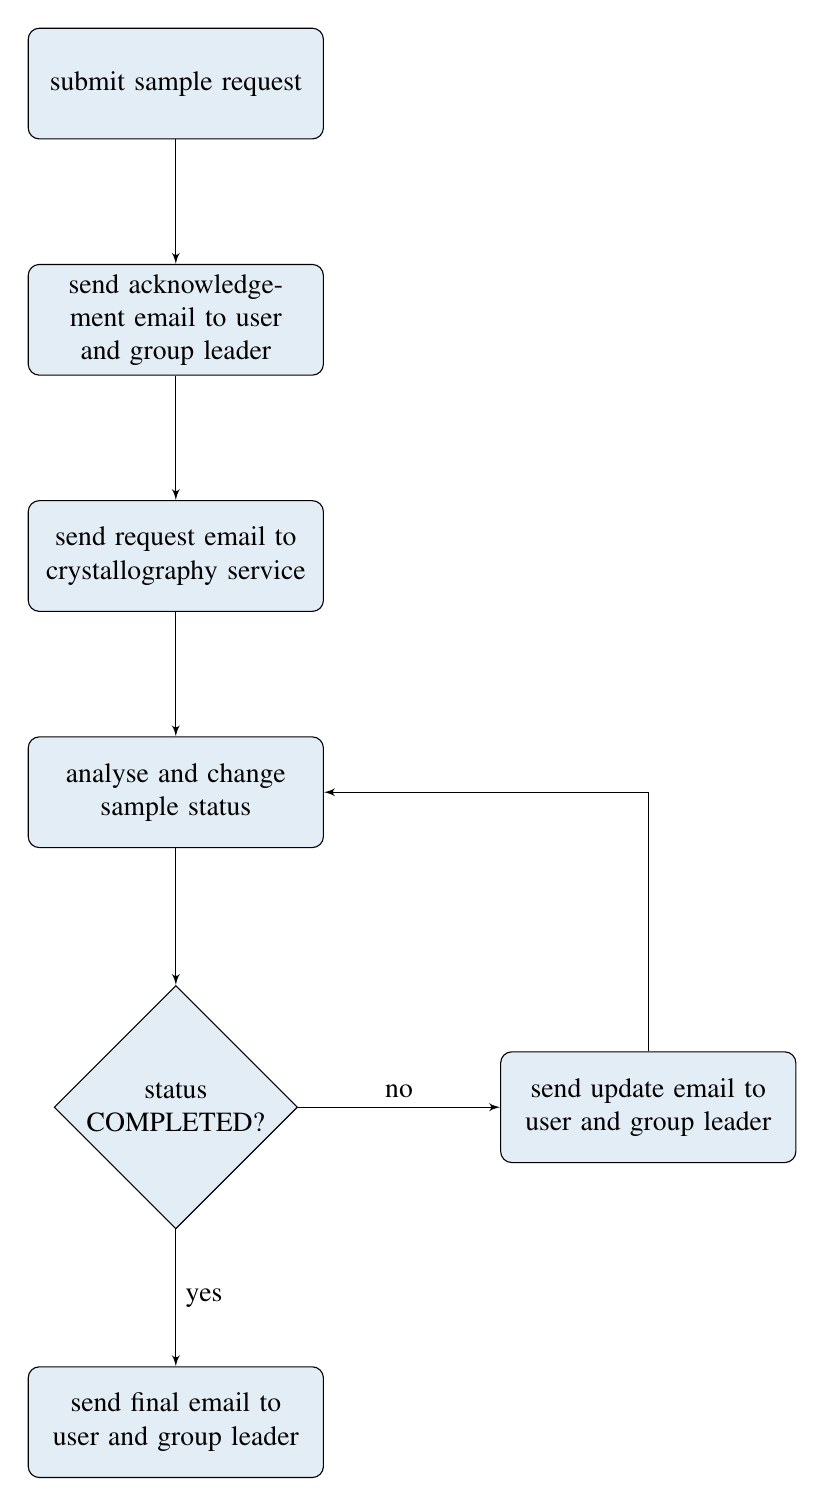
\begin{tikzpicture}[scale=2, node distance = 4cm, auto]
    % Place nodes
    \node [wideblock] (init) {submit sample request};
    \node [wideblock, below of=init, node distance=3cm] (email1) {send acknowledgement email to user
                                          and group leader};
    \node [wideblock, below of=email1, node distance=3cm] (email2) {send request email to
                                          crystallography service};
    \node [wideblock, below of=email2, node distance=3cm] (status) {analyse and change sample status};
    \node [decision, below of=status] (status1) {status\\COMPLETED?};
    \node [wideblock, right of=status1, node distance=6cm] (email4) {send update email to user
                                          and group leader};
    \node [wideblock, below of=status1] (email3) {send final email to user
                                              and group leader};
    % Draw edges
    \path [line] (init) -- (email1);
    \path [line] (email1) -- (email2);
    \path [line] (email2) -- (status);
    \path [line] (status) -- (status1);
    \path [line] (status1) -- node [, color=black] {no} (email4);
    \path [line] (status1) -- node [, color=black] {yes}(email3);
    \path [line] (email4) |- (status);
\end{tikzpicture}
\caption{Typical workflow for sample processing cycle.
Emails are sent automatically by the system whenever the status of a
sample is updated.\label{fig:sample_workflow}}
\end{center}
\normalsize
\end{figure}

\subsection{Public Pages}
Most information on the server can be viewed only by registered users.
However, there are some pages which are more generally accessible.
Such pages include the home page, general information pages and
the sample queue. Public pages can be created and edited by an administrator
using tools provided by the server software. rather than write pure
HTML, an administrator can use a text-based markup language called
\emph{Textile}\cite{textile}
which can produce sophisticated web pages with all the usual constructs
such as headings, paragraphs, floating elements, tables and images.

\section{Web Management Guide}
\subsection{Introduction}
In this section we describe the web management interface to the
sample tracking database. When a manager is logged-in, the home page of
the system looks similar to that shown in Figure \ref{fig:homepage}

\begin{figure}[!h]
\begin{center}
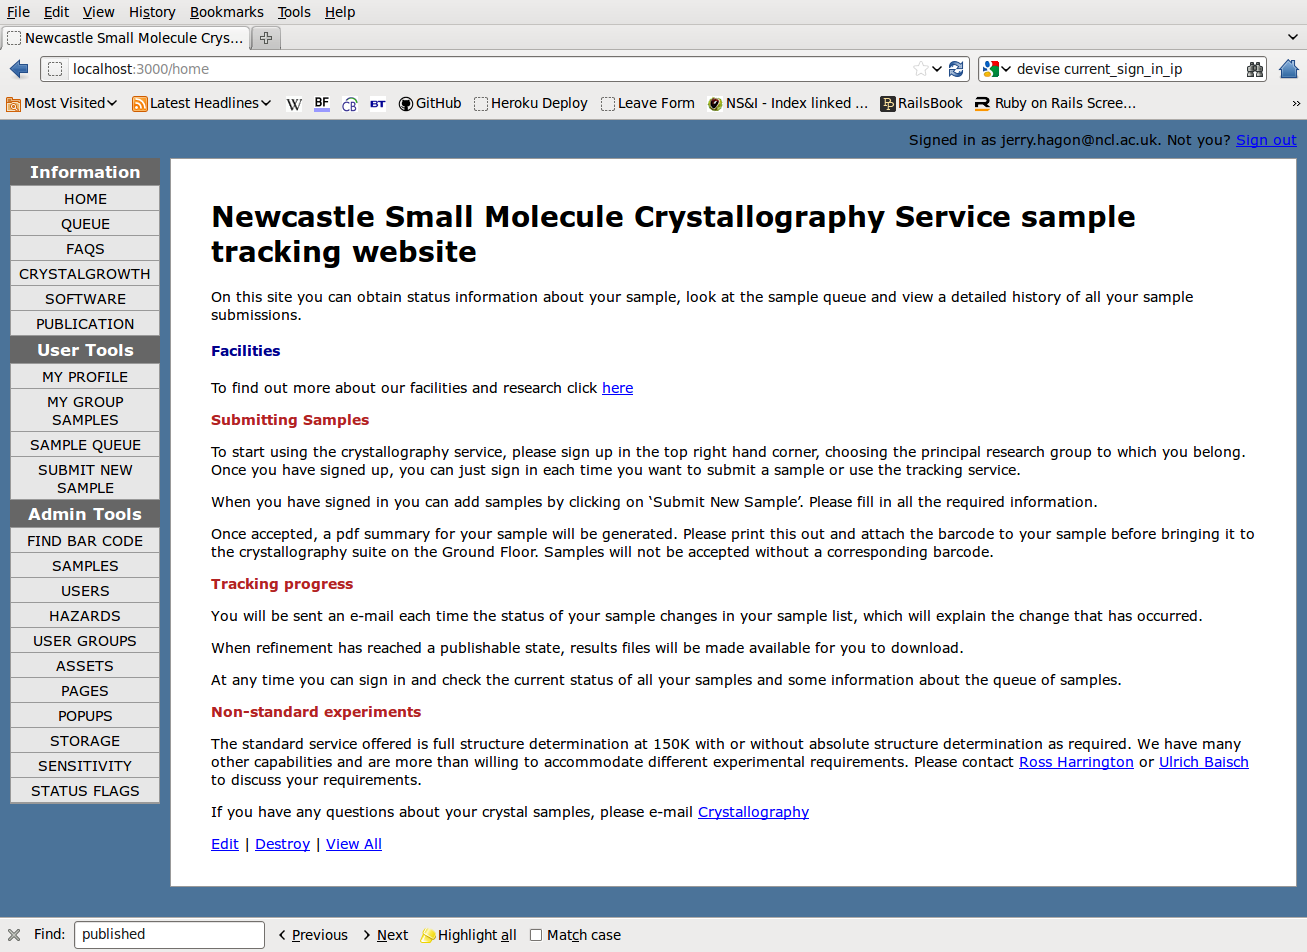
\includegraphics[width=0.75\textwidth]{homepage}
\caption{Administrator's view of home page.\label{fig:homepage}}
\end{center}
\end{figure}

There are three parts to this browser view:
\begin{enumerate}[(i)]
\item
a main display showing the contents of a page of information;
\item
a menu on the left side of the browser window;
\item
login information and a \verb=sign_out= link above the main display on
the right.
\end{enumerate}

The left side menu consists of three sections:
\begin{description}
\item[Information]
These links point to \emph{static} pages which can be created by an
administrator. the administrator can also add extra links to the
information section. We describe how to do this in \S\ref{sec:static}.
\item[User Tools]
These tools allow a user to view his sample list, submit a new sample
and view his profile information. Additionally, if a user is also a group
leader, he will have access to the \emph{My Group Samples} link for listing
all samples in the user's group.
\item[Admin Tools]
This is the main set of web-based tools for administrators. We will
describe each of these in the next section.
\end{description}
\subsection{Adding Static Pages}\label{sec:static}
Clicking the \emph{PAGES} link in the \emph{Admin Tools} sub-menu 
produces the pages index shown in Figure \ref{fig:pageidx}.
This shows a list of pages. For each of these pages is a set of buttons
allowing the administrator to show, edit or delete the page as shown in
Figure \ref{fig:showeditdelete}.
These buttons are used throughout the database editing pages on the web server.
At the bottom of the list is a link to create a new page.

\begin{figure}[!h]
\begin{center}

\includegraphics{show}\quad

\includegraphics{edit}\quad

\includegraphics{delete}
\end{center}
\caption{The \emph{show}, \emph{edit} and \emph{delete} buttons.
\label{fig:showeditdelete}}
\end{figure}

\begin{figure}[!h]
\begin{center}
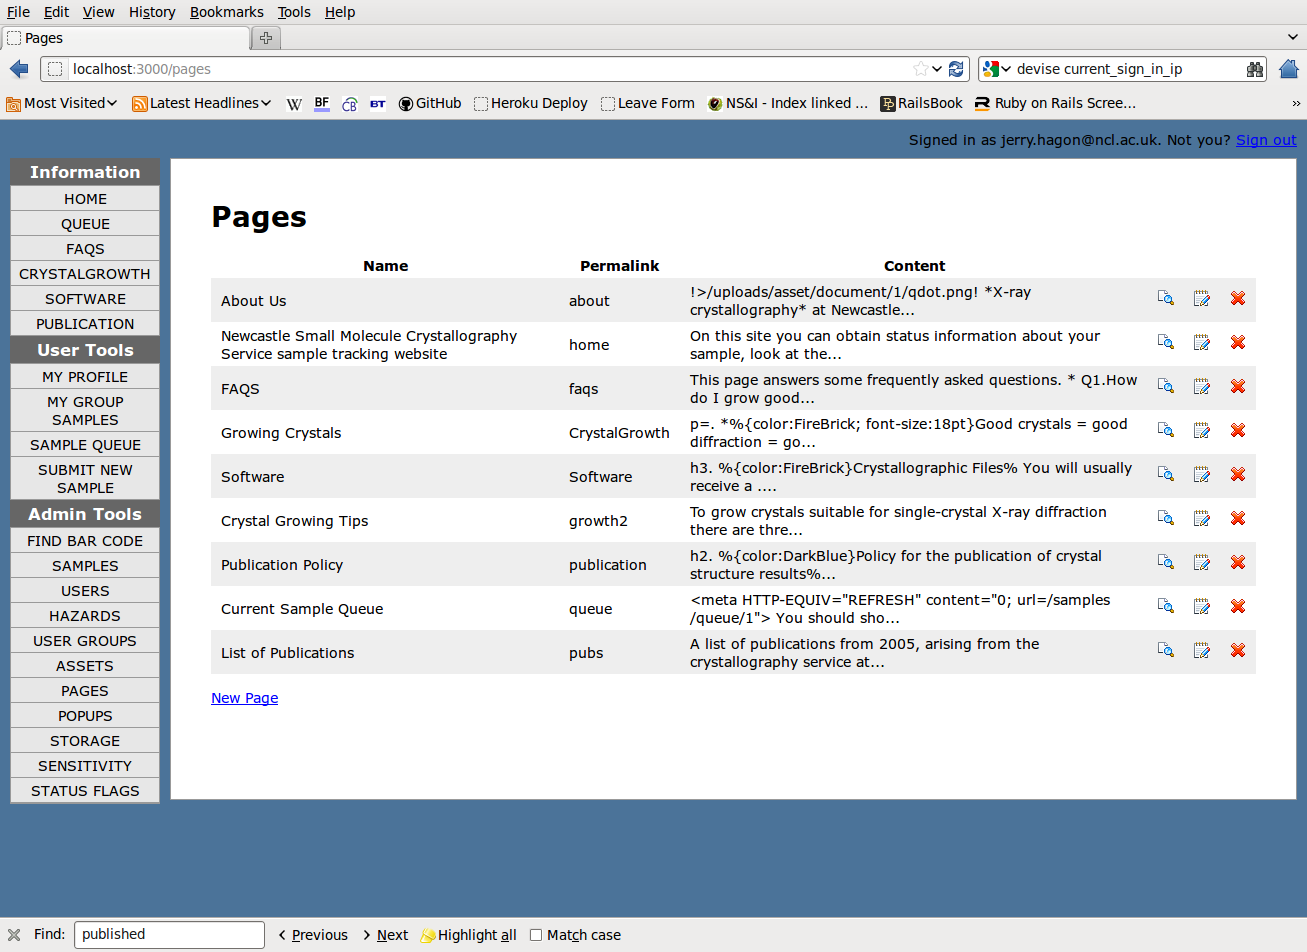
\includegraphics[width=0.75\textwidth]{pageidx}
\caption{The pages index view.\label{fig:pageidx}}
\end{center}
\end{figure}

\piccaption{The page edit view.\label{fig:editpage}}
\parpic[r]{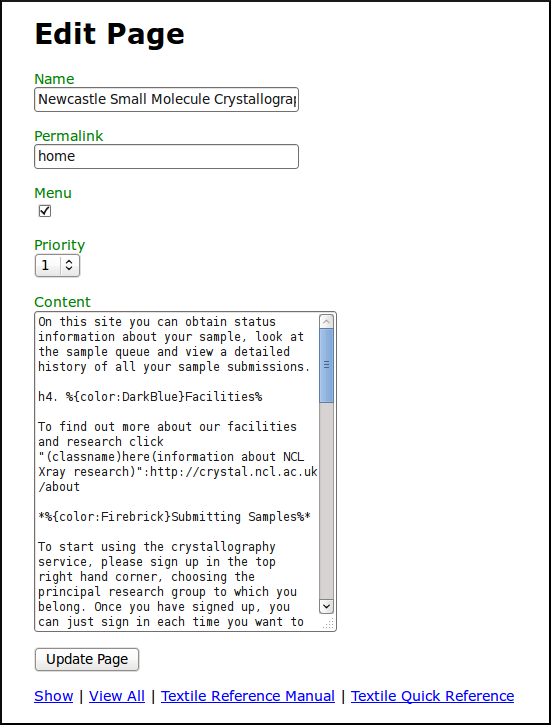
\includegraphics[width=0.4\textwidth]{editpage}}
Figure \ref{fig:editpage} shows the page editor --- a very simple form
for entering/changing text. This example shows the home page data. 
the content is entered in a markup language called Textile\footnote{You are 
allowed to mix HTML and Textile together.}. You can also specify the name
of the page (this will be used to set the HTML title attribute and a
permalink\footnote{A tag which is used as a basis for a concise URL.}.
At the bottom are links to the Textile Reference Manual, the page view
and the pages index. the page can be referred to via the URL:
\begin{verbatim}
<server name>/permalink
\end{verbatim}
thus making static page addressing very simple.
An alternative URL which can be generally used for any page is:
\begin{verbatim}
<server name>/pages/<id>
\end{verbatim}
but the permalink-based URL is what you'd almost always use in practice.
If, for some reason, you want to use the id-based URL, but don't know
what the id is, then just click the 'show' icon in the pages index for
the page you're interested in and look at the URL in the web browser window.

Note that there is also a checkbox labelled \emph{Menu}. If this is
checked then the page is added to the left hand \emph{Information} menu
of static pages. The \emph{Priority} parameter is an integer that
determines the order of the page in the menu. If two pages have the same
priority their order is determined alphabetically.
A good practice is to initially assign priorities in units of, say, 10.
Subsequently, if a new page is created, there are then plenty of 'spare'
priority numbers which can be used to add menu links in between
existing links --- otherwise existing priority numbers may need to be tweaked.

\subsection{Uploading General Files to the Server}
You can upload arbitrary files to the server. These files are referred
to as `assets' and can be uploaded via the \emph{ASSETS} link in the
\emph{Admin Tools} menu. Clicking on this link will take you to the
assets index page which looks very similar to the pages index described
in the previous section.
each index entry tells you the pathname of the file on the server,
together with a description of what the file contains. Often these files
will be images or documents (e.g. PDF files) that you want to link to
on one of the static web pages created as described in the previous
section.

At the bottom of the asset index list is a link to create a new asset.
Clicking this takes you to a simple menu where you can browse for a file
to upload to the server. Clicking the \emph{Create Asset} button will
then upload the file to the server. It will then be listed in the
asset index with an entry under the \emph{Document} column pointing
to its location in the file system. This location has the general form:
\begin{verbatim}
/uploads/asset/document/<id>/<filename>
\end{verbatim}
Here, \verb=<filename>= is the actual name of the uploaded file as it was
when it was uploaded. \verb=<id>= is the database id the document has
in the \verb=assets= table described in detail in \S\ref{sec:database}.
The actual URL of the document is then:
\begin{verbatim}
<servername>/uploads/asset/document/<id>/<filename>
\end{verbatim}

\subsection{Creating Users and Groups}
A user must belong to a group, so it is advisable to create a group for a
user before the user is created. Creating a user group is straightforward
via the \emph{USER GROUPS} link in the \emph{Admin Tools} menu.
As usual, this will take you to an index of existing groups, with a link
to create a new group at the bottom. Creating a new group merely requires
that you enter two fields:
\begin{enumerate}[(i)]
\item
a 3-letter group abbreviation (it \emph{must} be three letters);
\item
a longer group description.
\end{enumerate}

Users can be created in two ways; they can self-register by clicking
on the link top-right on the home page or they can be created by an
administrator. In either case the form used to create and register a new
user is the same.

\subsection{Sample Management}

In this section we give a complete description of the sample management
workflow.
\begin{enumerate}[(i)]
\item
First, a user fills out a sample submission form online. This form is
shown in Figure \ref{fig:sampleform}. This figure shows the
submission form from the point of view of both a non-administrative user
and an administrator.
\begin{figure}[!h]
\begin{center}
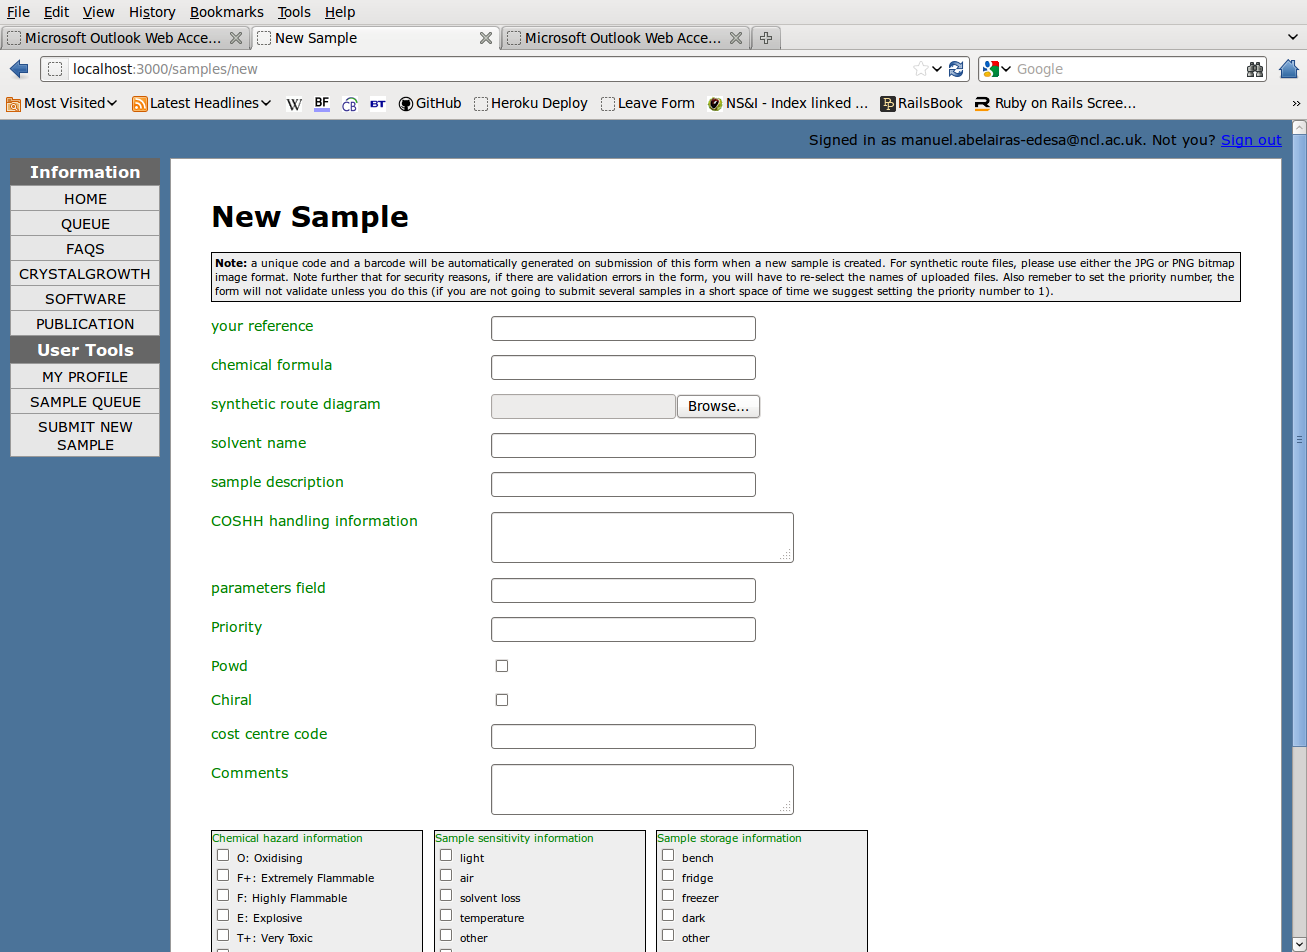
\includegraphics[width=0.45\textwidth]{sampleformuser}
\quad
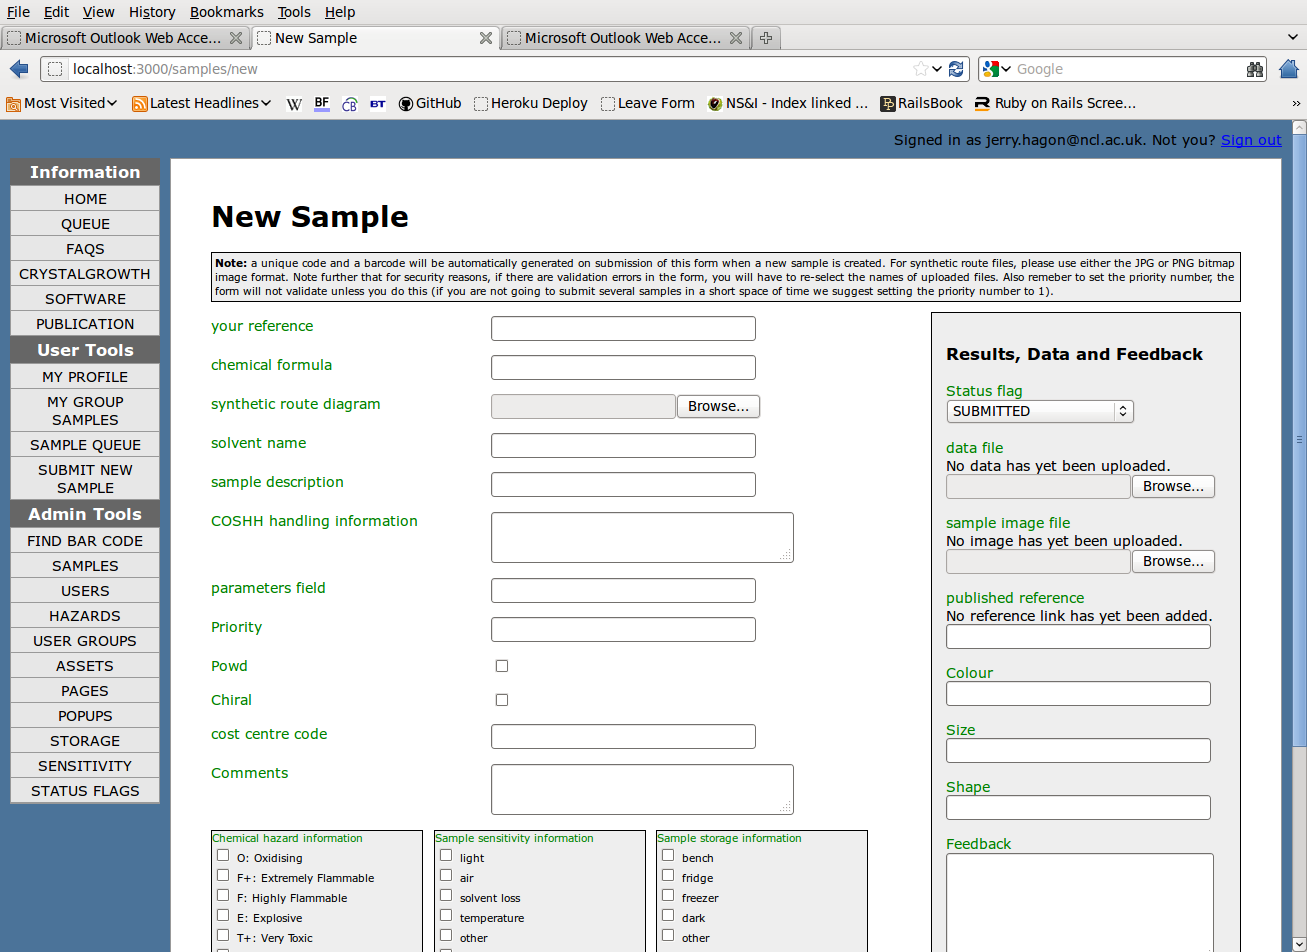
\includegraphics[width=0.45\textwidth]{sampleformadmin}
\caption{User's view (left) and administrator's view (right)
of the sample submission form.\label{fig:sampleform}}
\end{center}
\end{figure}

The bits that an ordinary user doesn't see are those parts of the sample
fields that are subsequently filled in by an administrator in the course
of sample processing.

There is a lot of validation built into the form making it very unlikely
that a form will be submitted with incomplete information.
Table \ref{table:samplevalidations} gives a complete list of
validation checks. If a validation check fails on submission of the form,
the user will be presented with the \emph{Invalid Fields} box which will
tell him which fields have not been entered correctly and what is
required. An extreme example of this is shown in Figure
\ref{fig:invalidfields} which shows what happens when none of the fields
in the form are filled-in.

\begin{figure}[!h]
\begin{center}
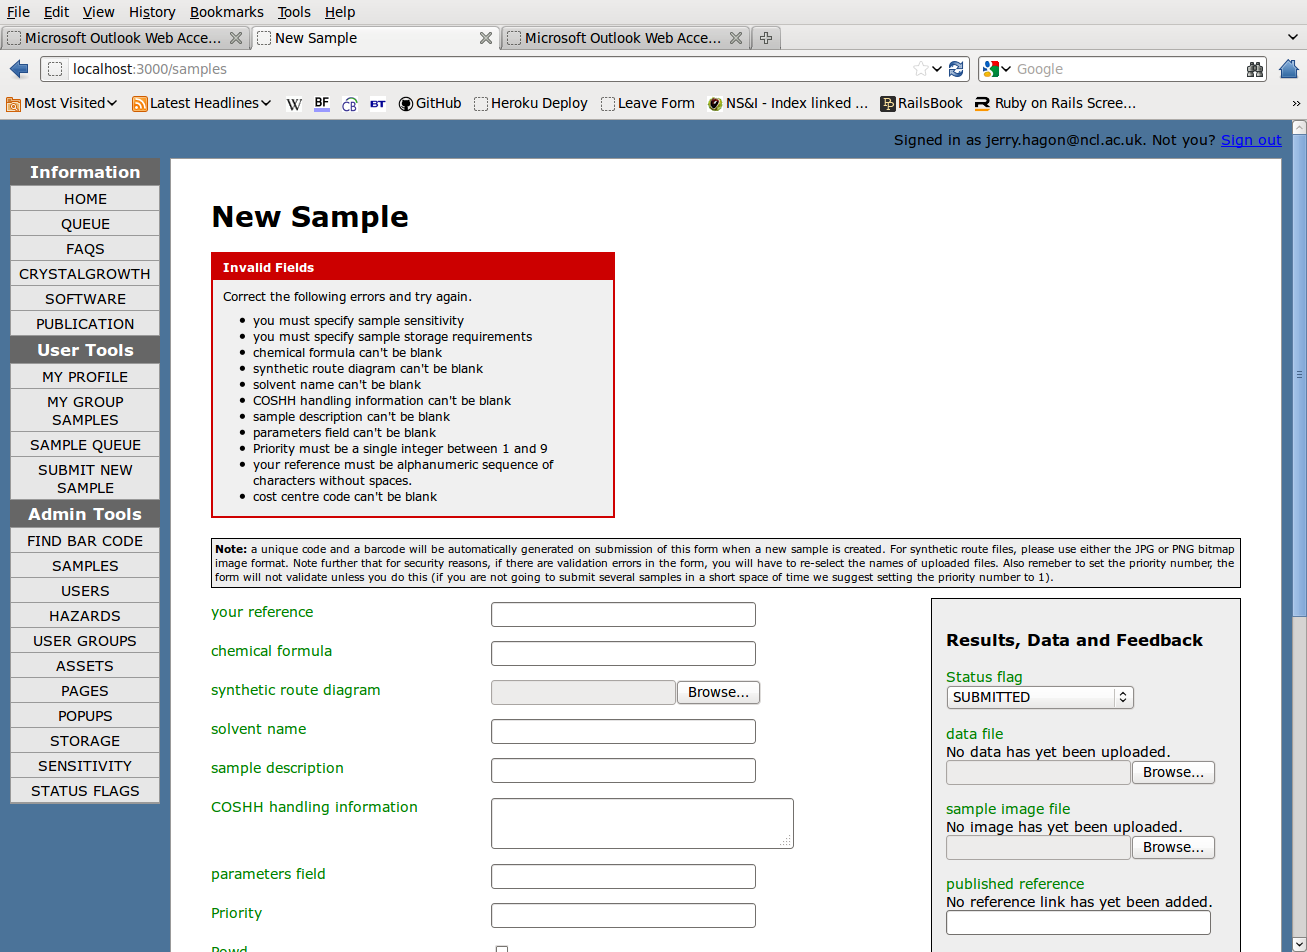
\includegraphics[width=0.45\textwidth]{invalidfields}
\quad
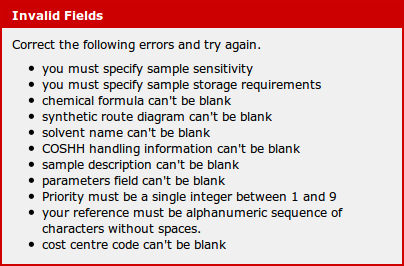
\includegraphics[width=0.45\textwidth]{invalidfieldsbox}
\caption{Illustrating what happens when an invalid form is submitted.
The user sees an \emph{Invalid Fields} box (shown enlarged on the right).
In this case, an administrative user has failed to fill in any of the fields
--- hopefully a very rare occurrence!\label{fig:invalidfields}}
\end{center}
\end{figure}

\item
On successful submission of the sample form, the user (and group leaders
if the user is not a group leader himself\footnote{If there is more than one
group leader then the other group leaders will also receive an email.}) 
will receive a confirmation email containing a link to the 
\emph{Sample Receipt} ---
a PDF file containing the user input information as well as a unique code
identifying the user, user group and sample and a unique barcode.
The email has the following general form with the tags in angle
brackets filled-in automatically:

\footnotesize
\begin{verbatim}
Dear User

New Sample Submission Code: <SAMPLE CODE> (your ref <SAMPLE USERREF>)
Submitted By: <USER FULL NAME>


your sample analysis request has been received. Please download a
receipt using the link below. Please quote the sample code in any
correspondence.

There is a tear-off slip at the bottom
of the receipt which you should attach to your sample.
You will be informed via email of any
changes in the status of your sample.

<LINK TO SAMPLE RECEIPT>

Copies of this email are sent to both sample submitters and their
research group leaders (where different).

Newcastle Crystallography Service
\end{verbatim}
\normalsize

A tear-off slip at the bottom of the sample receipt
containing the barcode, sample code and provided user
reference as well as essential COSHH information can be attached to the
actual sample itself.
Figure \ref{fig:samplereceipt} shows a typical sample receipt.

The receipt is generated on-the-fly from the supplied sample information. 
To perform the generation of the PDF, the well-known 
\href{http://prawn.majesticseacreature.com/}{Prawn} ruby library is used.
Once the sample has been submitted, a user can regenerate the sample receipt
at any time via a PDF link button in the sample list on his profile page
shown in Figure \ref{fig:userprofile}.

\begin{figure}[!h]
\begin{center}
\fcolorbox{darkgreen}{white}{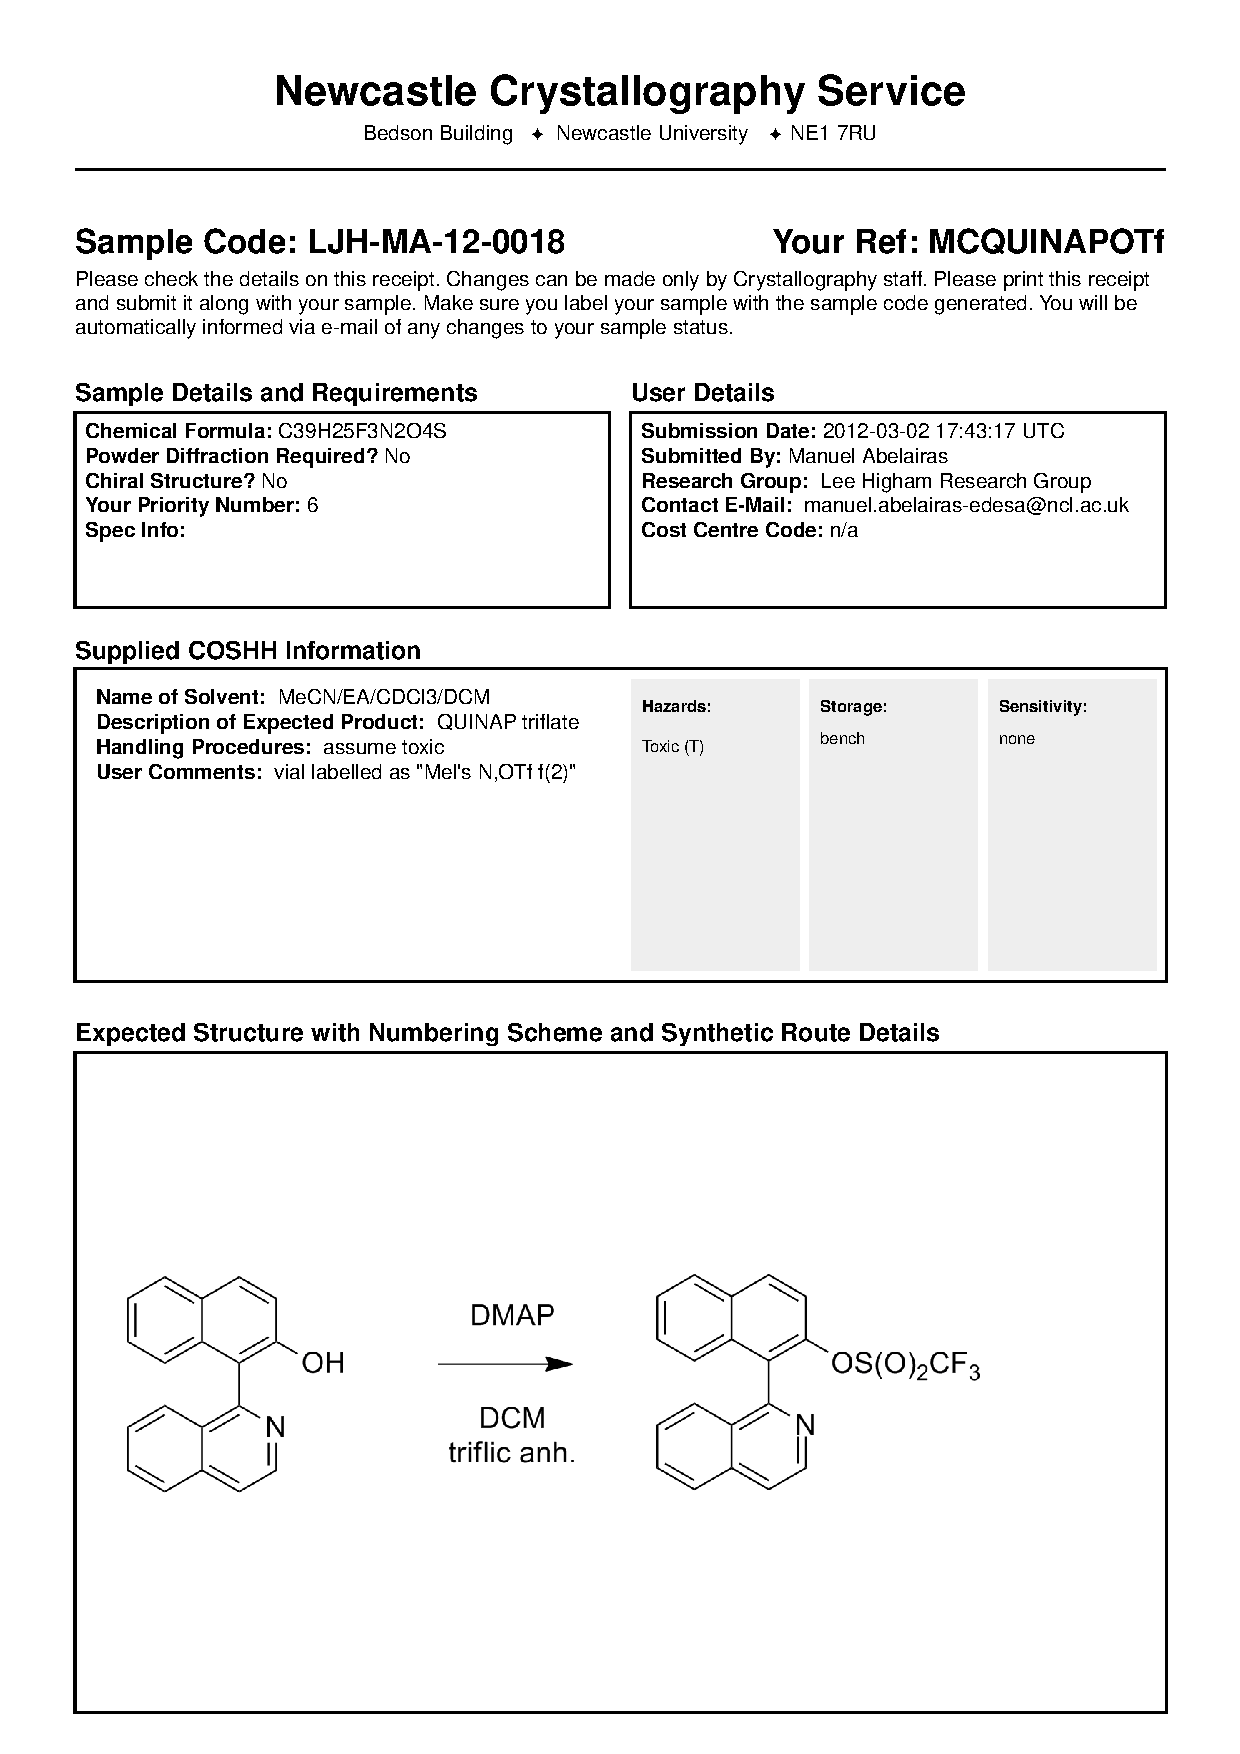
\includegraphics[width=0.9\textwidth]{samplereceipt}}
\caption{Example of a sample receipt (the actual size is A4).
Note the tear-off slip at the bottom. The receipt is generated
on-the-fly from the supplied sample information. The green border
is not part of the PDF rendering, it is used here merely to show
the A4 page border.\label{fig:samplereceipt}}
\end{center}
\end{figure}

\begin{figure}[!h]
\begin{center}
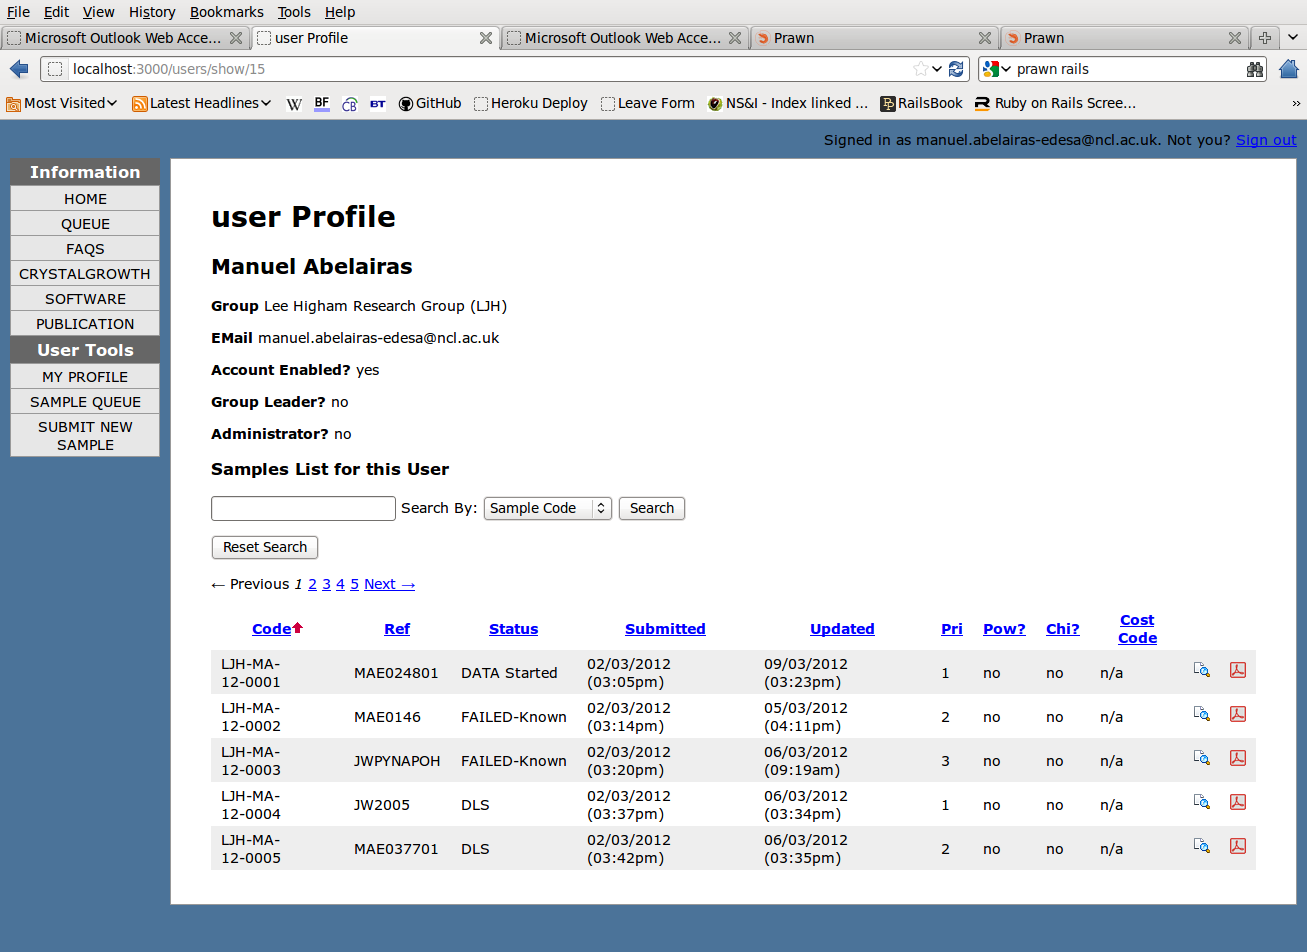
\includegraphics[width=0.65\textwidth]{userprofile}
\quad

\includegraphics{pdf.png}
\caption{User profile page showing sample list with PDF icon (shown
enlarged bottom right).\label{fig:userprofile}}
\end{center}
\end{figure}

\item
Next, the user brings his sample (with attached slip) for analysis and
at this point he should also see it in the sample queue.
\item
Initially the sample will have a status of \verb=SUBMITTED=. At various
points in the analysis, this status will be changed by crystallography
staff. Whenever the status is changed, an email is sent to both the user
and group leaders informing them of the change. The text of the email
looks similar to this:


\footnotesize
\begin{verbatim}
Dear User

This is to inform you that the status of sample
<SAMPLE CODE> (your ref <SAMPLE USERREF>) submitted by
<USER FULL NAME>
has changed as follows:

New Status: <NEW STATUS FLAG> <NEW STATUS FLAG DESCRIPTION>

Old Status: <OLD STATUS FLAG> <OLD STATUS FLAG DESCRIPTION>

<LINK TO FULL SAMPLE INFORMATION>

Copies of this email are sent to both sample submitters and their
research group leaders (where different).

Newcastle Crystallography Service
\end{verbatim}
\normalsize

\item
When crystallography staff have uploaded all results files (docx, res and
sample image) to the server and added any additional text feedback for
the sample, they will flag the sample as \verb=COMPLETED= and the process
will end. The sample data will continue to be available to users
(and administrators) indefinately after that.

Results files (docx and res) will usually be made available in a single 
zip file, with
the sample image in a separate file. The files are uploaded by
administrators using the sample edit form shown in 
Figure \ref{fig:sampleeditform}. Note that only administrators have access
to the sample edit form.
Users will see the information in a slightly different way, not as a form
but as a standard 'show' page. This view is shown in
Figure \ref{fig:sampleeditform}.Note that if administrators do not fill in the feedback section, then a
default message `No feedback given.' is seen on the relevant part of the
sample show page. This is also illustrated in 
Figure \ref{fig:sampleshowpage}.

\begin{figure}[!h]
\begin{center}
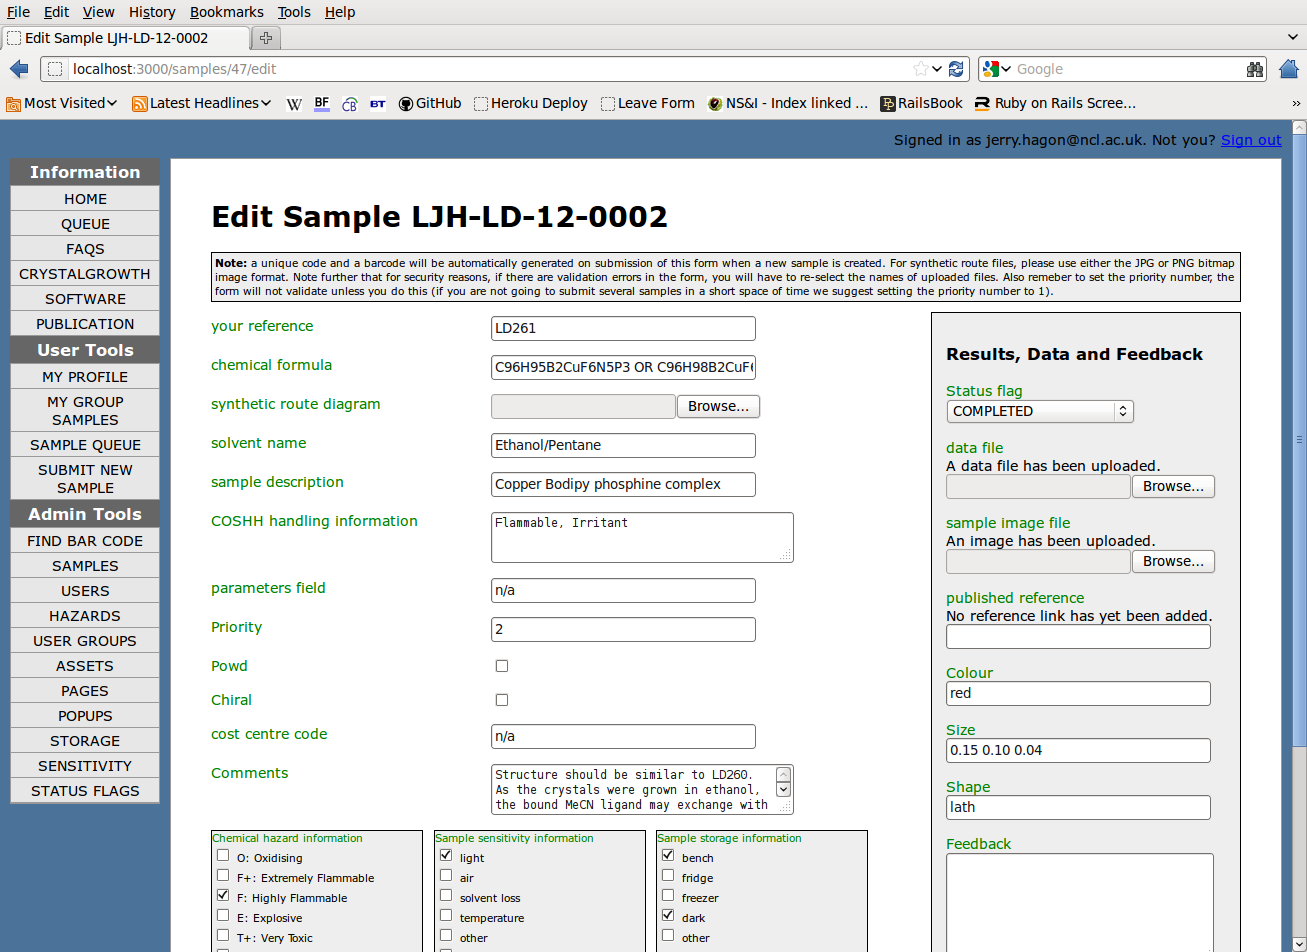
\includegraphics[width=0.75\textwidth]{sampleeditform}
\caption{A fully complete sample edit form.\label{fig:sampleeditform}}
\end{center}
\end{figure}

\begin{figure}[!h]
\begin{center}
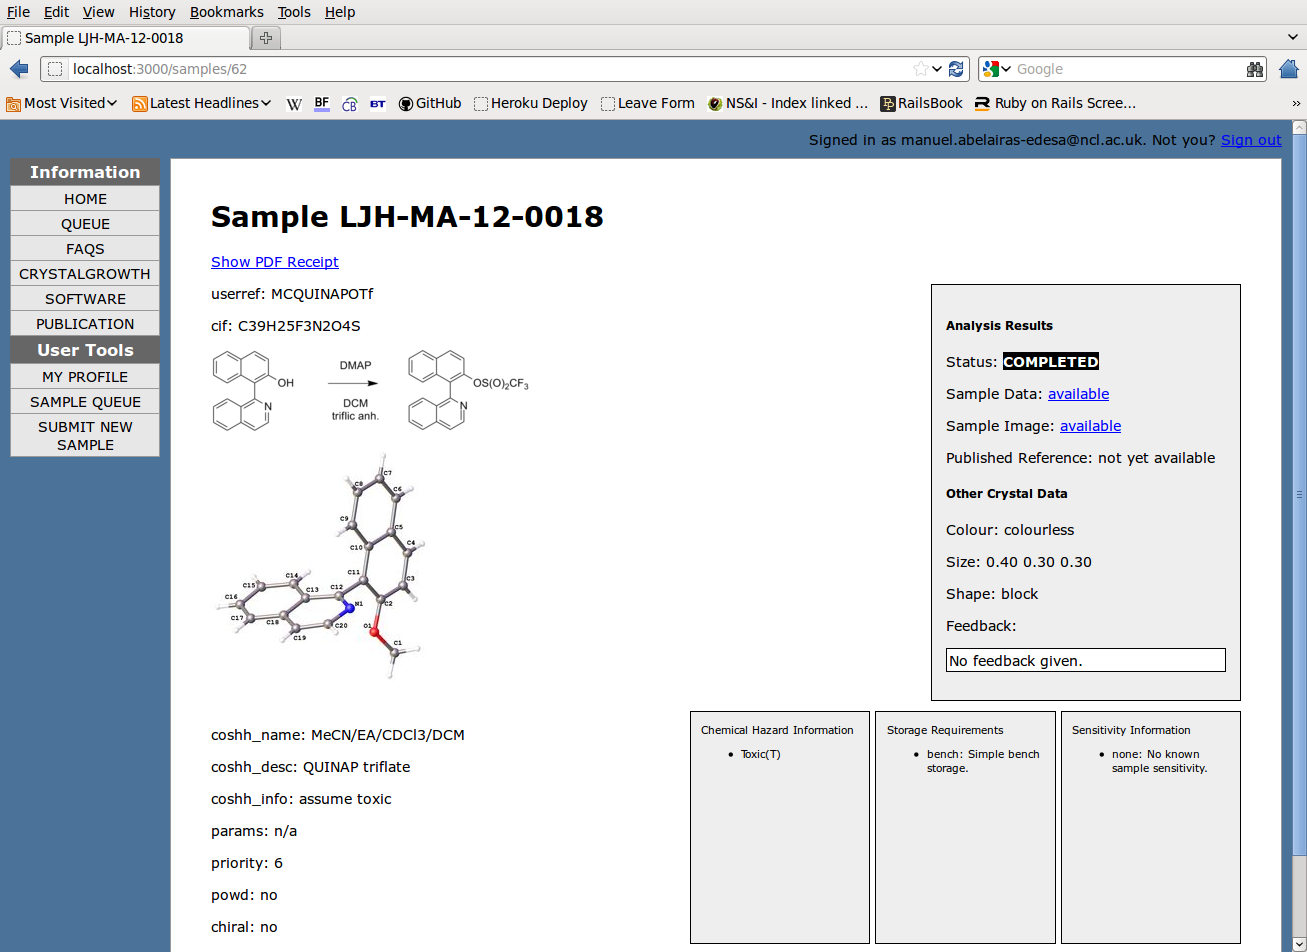
\includegraphics[width=0.60\textwidth]{sampleshowpage}
\quad
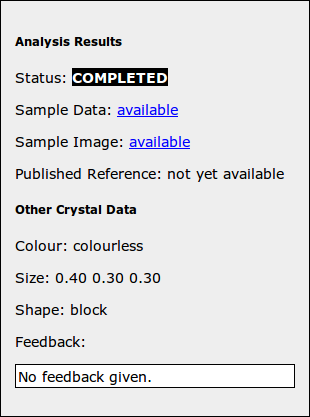
\includegraphics[width=0.30\textwidth]{sampleresults}
\caption{The user's view of a completed sample (left). On the right is
an enlarged view of the results section. Note also that a thumbnail image
of the sample is displayed. This thumbnail, when clicked, will show the
full-size image which can then be downloaded if desired.\label{fig:sampleshowpage}}
\end{center}
\end{figure}


\end{enumerate}

\subsection{Sample Search and Display Tools}
It is important that both administrators, group leaders and users can
find information about a particular sample or group of samples.
In this section we describe the tools that are available to quickly find
the sample data you need.

\begin{figure}[!h]
\begin{center}
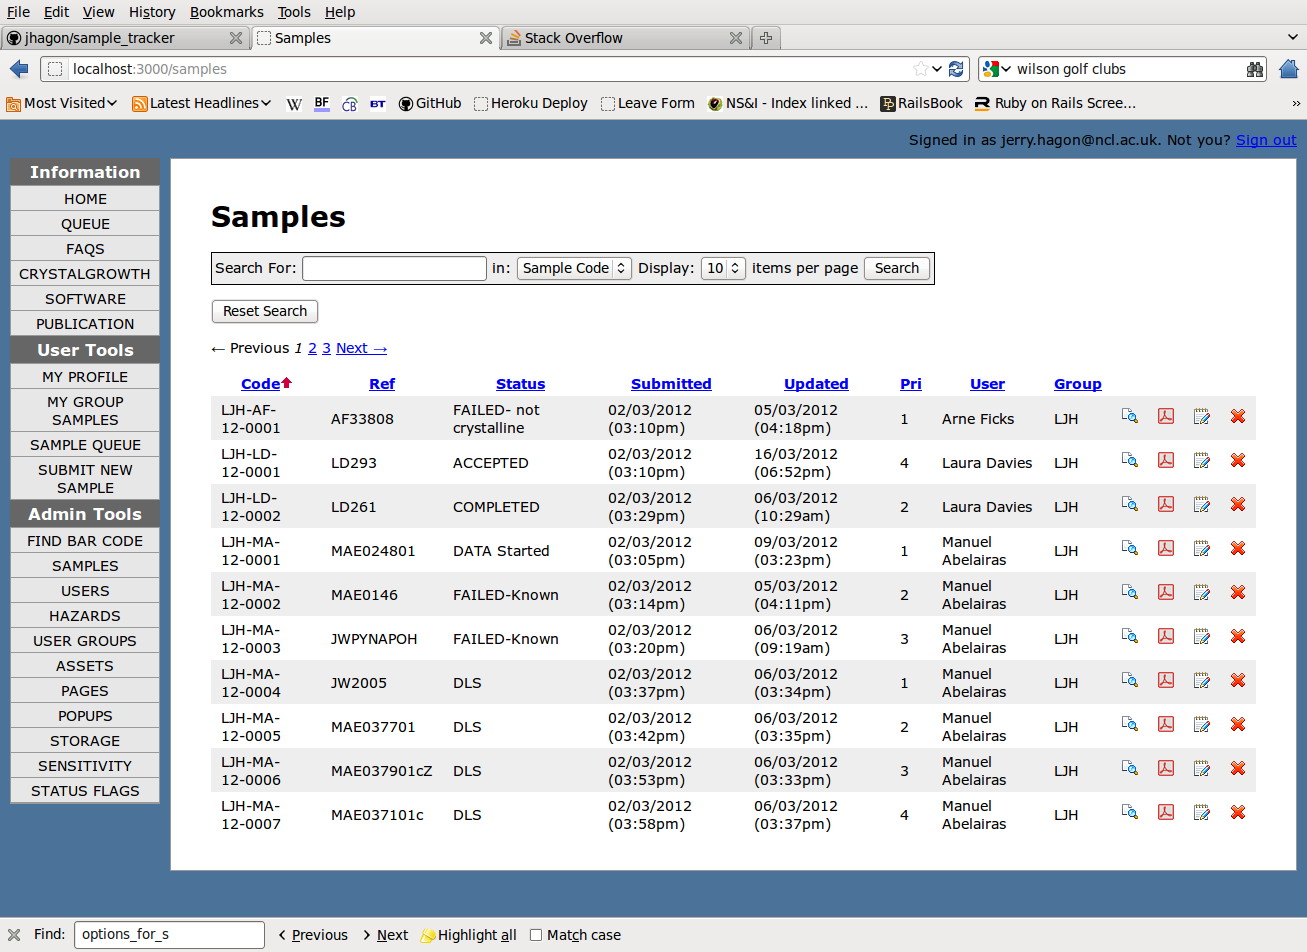
\includegraphics[width=0.75\textwidth]{sampleindex}
\caption{An administrator's view of the full sample index. 
In this case the red arrow next to the header in the \emph{Code}
column indicates that the list has been sorted by sample code in
ascending order (the default sorting).\label{fig:sampleindex}}
\end{center}
\end{figure}

For administrators, the usual starting point will be the main sample
index page shown in Figure \ref{fig:sampleindex}.
By default, this index is sorted by sample code in \emph{ascending} order.
This is indicated by a small red arrow pointing upwards next to the header
text in the \emph{Sample Code} column. 
Clicking the header text of the \emph{Sample Code} column will reverse the
order --- i.e. it will now be \emph{descending} order. This is indicated
by a blue arrow pointing downwards.
The list can be sorted on any other of the displayed columns simply by
clicking the column header. repeated clicking on the same column header
will toggle the sort order between ascending/descending.

The number of samples displayed per page can also be controlled by the
user. By default, this number is set by a global variable,
\verb=ITEMS_PER_PAGE= defined in the \verb=config/environment.rb= file\footnote{See the \emph{System Management} section for further details.}.
However, it can be easily changed by selecting the desired value from
a drop-down list in the search form above the sample list.
The first entry in this list is always the value in the
\verb=ITEMS_PER_PAGE= variable.
After the choice is made, the list will be re-paginated according to
the selected value. Note that for a full samples listing, the search box
itself must be empty when you do this.

\begin{figure}[!h]
\begin{center}

\includegraphics[width=0.75\textwidth]{searchform}
\caption{The sample index search form. This is usually found
above the list of samples in most of the sample index pages.
\label{fig:searchform}}
\end{center}
\end{figure}

To narrow down the list of samples you need to type something into
the search box in the search form above the sample list. This search form
is common to most of the sample listing pages and is shown in
Figure \ref{fig:searchform}.
Currently You can search on three fields: 
the sample code, the user reference or the status. When you perform
a search, the results will be paginated according to the setting of the
pagination parameter described above. Note that search results can be
sorted as before by clicking the header text of the column that you
wish to sort by.
Below the search form is a reset button which resets all the search
parameters (but not the pagination) to their default values.
You can also use the standard SQL \verb=%= symbol as a `wildcard'
character.

\begin{plainblock}
Note that searches are \emph{not} cumulative --- they are always made
with respect to the full set of samples. In other words if you perform
a second search after an initial search, the results of the second search
will be exactly the same as if it had been performed first.
\end{plainblock}

\subsubsection{BarCode Scanning}
\piccaption{A Zebex scanner.\label{fig:zebex}}
\parpic[r]{
\includegraphics[width=0.3\textwidth]{zebex}}
As mentioned earlier, each sample has associated with it a unique
barcode and it may sometimes be convenient to scan a sample barcode
and have the associated sample record displayed to the screen.
To this end, the system has a very simple interface which allows
a simple low-cost USB scanner such as the \emph{Zebex} scanner shown in 
Figure \ref{fig:zebex} to be used to extract a barcode.
The approach taken to facilitate this is brute force.

In the \emph{Admin Tools} menu is a link called \emph{Find Bar Code}.
Clicking this takes the user to a very simple form with just a single
entry field for a bar code. Now, assuming that the scanner is plugged in to
the same PC, if the mouse is clicked in the search box, then when the
scanner scans the barcode (usually a button needs to be pressed on the 
scanner) the actual code will magically appear in the box. Pressing
the search button on the form should then produce the matching sample
(see Figure \ref{fig:barcodeform}. 
For this to work correctly, the
barcode scanner needs to be put in \emph{keyboard emulation} mode.
Most scanners are capable of doing this, including the Zebex.
Of course, you can also type in the bar code by hand if you don't
have access to a scanner.

\begin{figure}[!h]
\begin{center}
\fcolorbox{darkgreen}{white}{%
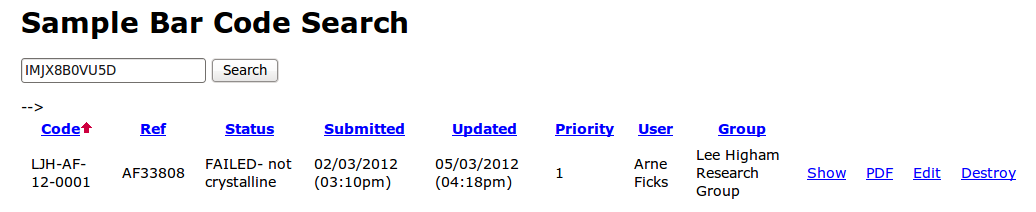
\includegraphics[width=0.75\textwidth]{barcodeform}}
\caption{A successful search using the \emph{Find Bar Code} form.
\label{fig:barcodeform}}
\end{center}
\end{figure}

\section{System Management and Internals}
\subsection{Introduction}
In this section we will explain lower-level aspects of the system
and its management.
This includes the operating system, command shell, web server, 
database, ruby language, ruby gems, and the rails3 system which is
used to do most of the programming.

\subsection{Basic Components of the System}
To begin with, we will describe the components of the system from the
operating system right up to the \emph{Rails3} software which is used
to write the web interface to the sample database.
Figure \ref{fig:systemcomponents} summarizes the main components and
their relationships.

\begin{figure}[!ht]
\small
\begin{center}
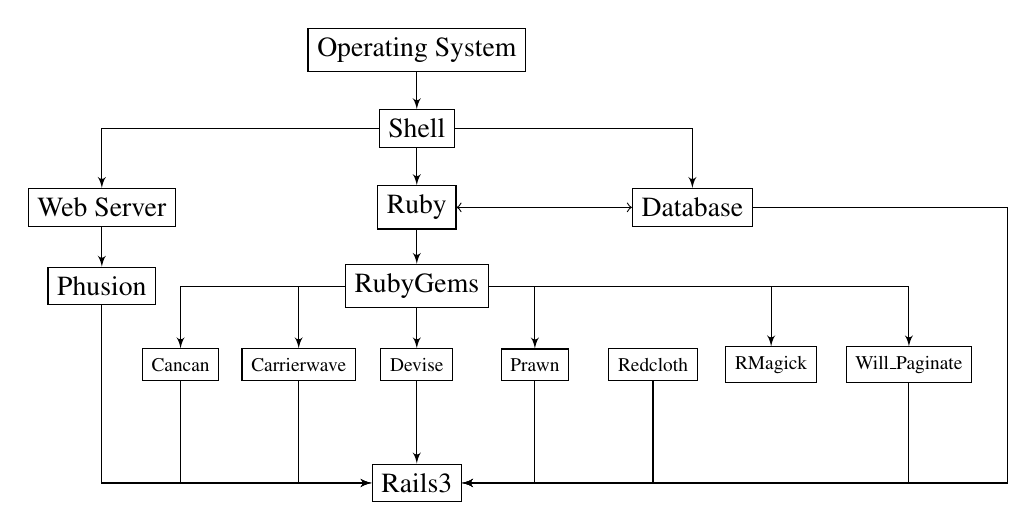
\begin{tikzpicture}
\node (os) at (0,1) [draw] {Operating System};
\node (shell) at (0,0) [draw] {Shell};
\node (web) at (-4,-1) [draw] {Web Server};
\node (database) at (3.5,-1) [draw] {Database};
\node (ruby) at (0,-1) [draw] {Ruby};
\node (phusion) at (-4,-2) [draw] {Phusion};
\node (gems) at (0,-2) [draw] {RubyGems};
\node (cancan) at (-3,-3) [draw] {\scriptsize Cancan};
\node (cwave) at (-1.5,-3) [draw] {\scriptsize Carrierwave};
\node (devise) at (0,-3) [draw] {\scriptsize Devise};
\node (prawn) at (1.5,-3) [draw] {\scriptsize Prawn};
\node (redcloth) at (3.0,-3) [draw] {\scriptsize Redcloth};
\node (rmagick) at (4.5,-3) [draw] {\scriptsize RMagick};
\node (willp) at (6.25,-3) [draw] {\scriptsize Will\_Paginate};
\node (rails) at (0,-4.5) [draw] {Rails3};
% draw lines
\path [line] (os) -- (shell);
\path [line] (shell) -| (web);
\path [line] (shell) -| (database);
\path [line] (shell) -- (ruby);
\path [line] (web) -- (phusion);
\path [line] (ruby) -- (gems);
\path [line,<->] (ruby) -- (database);
\path [line] (gems) -| (prawn);
\path [line] (gems) -| (cwave);
\path [line] (gems) -- (devise);
\path [line] (gems) -| (cancan);
\path [line] (gems) -| (rmagick);
\path [line] (gems) -| (willp);
\path [line] (phusion) |- (rails);

\path [line] (prawn) |- (rails);
\path [line] (cwave) |- (rails);
\path [line] (devise) -- (rails);
\path [line] (cancan) |- (rails);
\path [line] (willp) |- (rails);
\path [line] (redcloth) |- (rails);

\path [line] (database) -- (7.5,-1) |- (rails);
\end{tikzpicture}
\end{center}
\normalsize
\caption{The main components of the sample tracking system and their
relationships. This diagram takes a `top-down' view starting with
the operating system and moving through the various software layers
down to the rails3 system itself on which the sample tracking software
is based.\label{fig:systemcomponents}}
\end{figure}

Let's now look at each of these components individually:
\begin{description}
\item[Operating System]
The system runs on a computer running the Ubuntu version of the
linux operating system.
The specific release used at present is \emph{Ubuntu 10.04.3 LTS}.
Release 10.04 is also known via the codename `lucid'. LTS stands
for 'Long Term Support'. Extended support for this version will
last until 2014.
\item[Shell]
Access to most software on linux is vis a command shell. There are
many different shells available, the default being the \emph{bash}
shell. We will assume the use of bash throughout this guide, but
other shells can be also be used with little, if any modification
to the software itself.
\end{description}

Running under the shell are the three principal components of
the system: a web server, database and the ruby programming language
environment.
\begin{description}
\item[Web Server]
The web server we use is the ubiquitous \emph{Apache}, specifically
version 2.2.14.
\item[Ruby]
The version of ruby that comes with Ubuntu 10.04.3 is 1.8.7.
Unfortunately, this version is not recent enough to run a rails3
application. So, we use the \emph{Ruby Version Manager} to run a more
recent version of ruby (1.9.2).
\item[Database]
Rails 3 requires a database application to store and retrieve sample data.
We are using the \emph{SQLite3} database. This is a `lightweight' database
which requires very little separate maintenance. In particular, it
does not require a separate authentication process for acces, nor
does it need to run a separate process in the background as with other
database software such as \emph{mysql}.
\end{description}

There are two other components of the system which sit between the
web server, ruby and database layer:

\begin{description}
\item[Phusion Passenger]
is an Apache module -- a `plugin' -- which
interfaces a rails3 application to the Apache web server. It also supplies
some debugging and error logging information which can be useful when
things go wrong.
\item[Ruby Gems]
are extension libraries to ruby. Some of them are
specific to rails3, but most have wider applicability and can be used in
more general applications. The ruby gems used in the sample tracking
application are described in the next section.
\end{description}

\subsubsection{Ruby Gems}
The following Ruby Gems are used in the application:
\begin{description}
\item[cancan\cite{cancan}]
written by well-known Rails programmer Ryan Bates is used for
authorization. By this we mean controlling which parts of the application
can be accessed by users. For example, some parts of the application can
be accessed only by administrative users and others can be accessed by
anyone --- even those who have not registered to use the system.
\item[carrierwave\cite{carrierwave}]
is used to manage the upload of various files to the application
including data files, image files and general asset files.
\item[devise\cite{devise}]
is an authentication plugin to Rails which handles user data and
user authentication. It provides related functionality such as forgotten
password recovery (via email), user login statistics and more.
\item[prawn\cite{prawn}]
is a ruby library for producing PDF files. It is used to
auto-generate the sample receipts.
\item[redcloth\cite{redcloth}]
is a Ruby library used for parsing and display of Textile input.
\item[rmagick\cite{rmagick}]
is a well-known software application consisting of both
libraries and utility programs for manipulation of bitmap graphic files.
This gem interfaces the ImageMagick libraries to Ruby allowing
ImageMagick routines to be called from within a Ruby program.
\item[will\_paginate\cite{willp}]
is used to set up pagination of sample listings (and other things).
\end{description}

\subsection{Web Server Management}
Most of the time, you should need only
two commands when managing the web server --- the commands to switch it on
and off. To do this use:
\begin{verbatim}
sudo apache2ctl start|stop
\end{verbatim}
You would typically stop the server to do some maintenance such as editing
a stylesheet or a major upgrade to the software.
Occasionally you may need to change some server parameters in the
web server configuration files. The main configuration file is
\verb=/etc/apache2/apache2.conf=. You will rarely, if ever, need to
change anything here unless you want to tweak the server performance (in
which case you'll definately need to know what you're doing). This file
does contain some parameters for the apache \emph{Phusion Passenger} 
module which is needed to interface Rails with the apache server:
\begin{verbatim}
LoadModule passenger_module /usr/local/rvm/gems/ruby-1.9.2-p290/
gems/passenger-3.0.9/ext/apache2/mod_passenger.so
   PassengerRoot /usr/local/rvm/gems/ruby-1.9.2-p290/gems/passenger-3.0.9
   PassengerRuby /usr/local/rvm/wrappers/ruby-1.9.2-p290/ruby
\end{verbatim}
These configuration lines are added as part of the installation of
\emph{Phusion Passenger} and tell it where the ruby interpreter and
passenger software reside in the file system.

The \verb=apache2.conf= file also contains a line which refers to some other
configuration files:
\begin{verbatim}
Include /etc/apache2/sites-enabled/
\end{verbatim}
The above line tells the server to get some further configuartion
details from the contents of the directory
\verb=/etc/apache2/sites-enabled=.
\verb=sites-enabled= contains a file called \verb=000-default= which contains
the descriptions of all the \emph{virtual hosts}\footnote{A single Apache
web server can support multiple so-called virtual hosts which behave as
separate web sites.}. The most important virtual host entry is the one
for the host \verb=crystal.ncl.ac.uk=. Here is the entry in full:
\begin{verbatim}
<VirtualHost *:80>
      ServerName crystal.ncl.ac.uk
      DocumentRoot /usr/local/share/sample_tracker/public
      <Directory "/usr/local/share/sample_tracker/public">
         AllowOverride all
         Options -MultiViews
      </Directory>
        ErrorLog /var/log/apache2/error-crystal.log
</VirtualHost>
\end{verbatim}
For virtual hosting to work, any name given to a virtual host
(e.g. in this case \verb=crystal.ncl.ac.uk=) must be an official alias
for the actual apache web server (in this case \verb=milkyway.ncl.ac.uk=).
We will now describe in detail what these directives mean.

The first line is a tag which defines the beginning of a virtual host
definition. It has the form \verb=<VirtualHost *:80>=. The number \verb=80=
is the \emph{port number}\footnote{A port number defines a communications
channel between computers on the Internet. Port 80 is usually
used by the HTTP protocol for communication between web servers and browsers
although other port numbers can be used.}.
The last line is a closing tag, \verb=</VirtualHost>=. the lines in-between
contain the directives which control the configuration of this host.
\begin{description}
\item[\texttt ServerName]
This directive sets the name of the virtual host, in this case
\verb=crystal.ncl.ac.uk=.
\item[\texttt DocumentRoot]
Sets the absolute path of the directory on the server which contains
all static documents which can be \emph{directly} viewable on a web browser.
No documents outside this directory can be viewed directly or downloaded.
In this case, the document root is 
\verb=/usr/local/share/sample_tracker/public=
i.e. the \verb=public= directory within the full sample tracking application.
This is a standard rails convention.
\item[\texttt ErrorLog]
Specifies the absolute path of the error log file for this virtual host.
Here, it is set as \verb=/var/log/apache2/error-crystal.log=.
\end{description}
There is also a \verb=Directory= section in the virtual host definition.
This has the form of an opening and closing tag with directives in-between.
The opening tag has an argument which is the full path of the particular
directory to which the directives apply. Note that the argument is in quotes.
In this case the argument is the same directory as the document root.
Note further that there may be more than one \verb=Directory= section.
The directives are as follows:
\begin{description}
\item[\texttt AllowOverride]
This directive controls whether directives contained in a file
(conventionally called \verb=.htaccess= contained in a particular
directory can override earlier configuration directives at the server
configuration level. The argument refers to which type of directive
can be overridden --- in this case \verb=all=.
\item[\texttt Options]
This sets a number of options when viewing files contained in the
relevant directory. here, we have set the \verb=-MultiViews= option
which allows a single document to be displayed in different ways dependent
on browser capabilities.
\end{description}

\begin{plainblock}
\begin{center}
\bfseries Location of the Sample Tracking Application
\end{center}
It should be clear from the above that if you want to change the
location of the sample tracking application you must edit the
virtual host directive file and change the \verb=DocumentRoot= directive
and \verb=Directory= section argument appropriately.
\end{plainblock}

We end this section on web management with a brief discussion about
file permissions. Once you have uploaded the application and all its
files to a suitable location you must make sure that the file permissions
are correct. The correct permissions for all files are to set group
ownership to \verb=root= and user ownership to \verb=nobody=\footnote{%
\texttt{nobody} is a special user account available on most linux
systems.}. This can be done with a simple one-line command:
\begin{verbatim}
sudo chown -R nobody.root <application document root>
\end{verbatim}

\subsection{Application File and Directory Management}
In this section we describe the overall file and directory structure
of the application. Some of the files contain parameters which can be
changed to affect the behaviour of the application or the appearance
of the views. The overall directory structure is shown in
Figure \ref{fig:filestructure}.

\begin{sidewaysfigure}
\captionsetup{width=10cm}
\begin{center}
\scriptsize
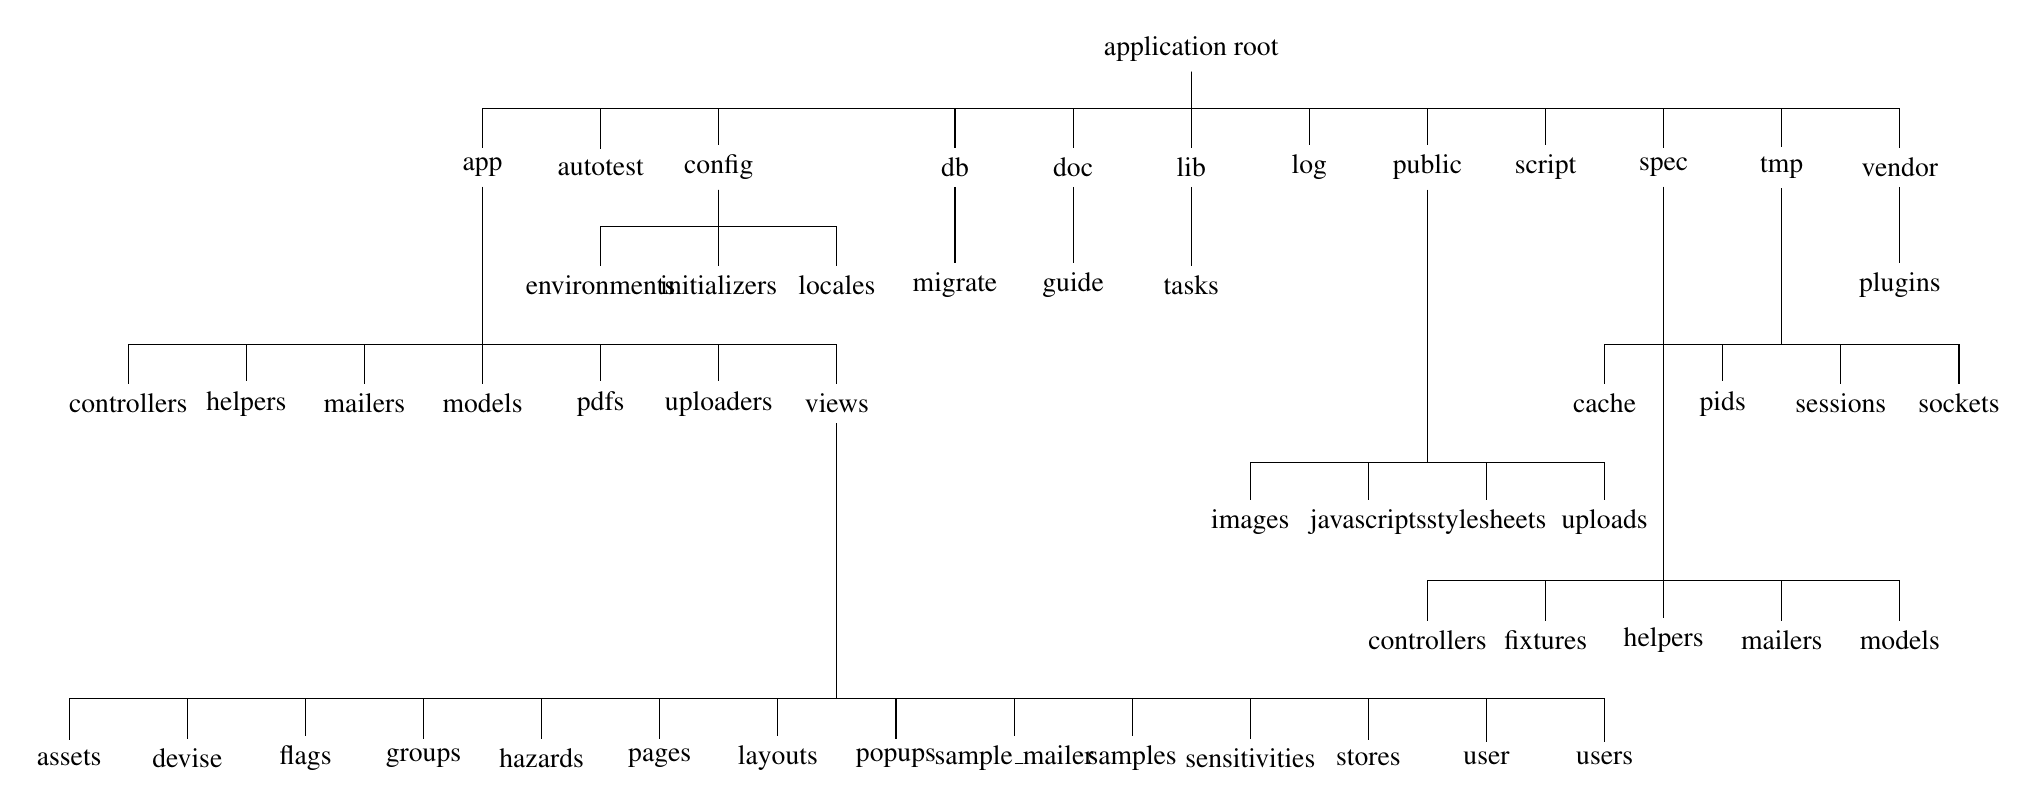
\begin{tikzpicture}
\node (root) {application root}
  [edge from parent fork down]

  child {node {app}
  child {
    child {node {controllers}}
    child {node {helpers}}
    child {node {mailers}}
    child {node {models}}
    child {node {pdfs}}
    child {node {uploaders}}
    child {node {views}
    child {
    child {
      child {node {assets}}
      child {node {devise}}
      child {node {flags}}
      child {node {groups}}
      child {node {hazards}}
      child {node {pages}}
      child {node {layouts}}
      child {node {popups}}
      child {node {sample\_mailer}}
      child {node {samples}}
      child {node {sensitivities}}
      child {node {stores}}
      child {node {user}}
      child {node {users}}
}
}
}
}
}
%  child [missing] {}
  child {node {autotest}}
  child {node {config}
    child {node {environments}}
    child {node {initializers}}
    child {node {locales}}
}
  child [missing] {}
  child {node {db}
    child {node {migrate}}
}
  child {node {doc}
    child {node{guide}}
}
  child {node {lib}
    child {node{tasks}}
}
  child {node {log}}
  child {node {public}
  child {
  child {
    child {node {images}}
    child {node {javascripts}}
    child {node {stylesheets}}
    child {node {uploads}}
}
}
}
  child {node {script}}
  child {node {spec}
  child {
  child {
  child {
    child {node {controllers}}
    child {node {fixtures}}
    child {node {helpers}}
    child {node {mailers}}
    child {node {models}}
}
}
}
}
  child {node {tmp}
  child {
    child {node {cache}}
    child {node {pids}}
    child {node {sessions}}
    child {node {sockets}}
}
}
  child {node {vendor}
    child {node {plugins}}
}
;
\end{tikzpicture}
\normalsize
\end{center}
\vspace{1cm}
\caption{The application directory structure. Only directories are
shown here. See text for a detailed explanation.
\label{fig:filestructure}}
\end{sidewaysfigure}

The application root directory contains the following files:
\begin{verbatim}
config.ru Gemfile Gemfile.lock README.markdown
\end{verbatim}
\verb=README.markdown= is a brief summary of the application, written in
\emph{markdown}, a simple markup language similar to Textile. The
contents of this file are automatically displayed when viewing the home
page of the application on GitHub.

\verb=config.ru= is a file used to initialize the application via a
special software interface called \emph{Rack}\footnote{Rack is part
of the interface between a rails application and a web server.}.

\verb=Gemfile= contains a list of gems required to run the application.
\verb=Gemfile.lock= contains a list of all gems and their dependencies
and is used to update or install additional gems for the application.
In practice, only the \verb=Gemfile= is actually edited.

\section{The Database}\label{sec:database}
\subsection{Introduction}
The core of the system is the database which holds information about 
users, samples etc. In this section we describe the whole database
structure (or \emph{schema} in database parlance).
The easiest way to get an overall view of the database schema is to
study Figure \ref{fig:database_schema}. This shows
all the tables, fields and relationships in a single diagram.
We now give a brief description of each table.

Note that all tables except join tables have an autoincremented integer field
called \verb=id= which servers as the unique primary key for each record
in the table. The \verb=id= field will not be listed explicitly in the
description of each table. All non-join tables also have two other
fields, \verb=created_at= and \verb=updated_at= in a datetime format.
Again, we will not explicitly list these fields in the description
of the tables which follows.

\subsection{The Samples Table}
The samples and users tables are the key parts of the database as is
evident from Figure \ref{fig:database_schema}. They are related to each
other via a \emph{one-to-many} relationship, i.e. \emph{one} user
can have \emph{many} samples. The samples table
consists of the following fields:
\begin{description}
\item[code]
a string, automatically generated by the system having the
general form \verb=AAA-AA-YY-1111= where the \verb=AAA= and \verb=AA= 
represent 3-letter codes for group and submitter respectively; 
the \verb=YY= represents the year and the \verb=1111= represents a number 
which is incremented for that group but reset to zero at the start of each 
calendar year.
\item[cif]
a string representing the chemical formula of the sample in cif format.
\item[synth]
a string representing the file name of an image file specifying the details
of the synthesis.
\item[coshh\_name]
a string representing the name of the solvent (if any).
\item[coshh\_info]
another string describing any procedures in case of contact with the sample.
\item[coshh\_desc]
a text field providing a brief description of the sample (e.g. organic amide).
\item[params]
a string representing unit cell parameters
or CSD/Newcastle code for possible by-products or previously obtained, 
unpublished results.
\item[priority]
an integer between 1 and 9 to give an indication of priority.
\item[powd]
a boolean parameter indicating if the sample requires powder diffraction (y/n).
\item[chiral]
another boolean indicating whether the molecule is chiral (y/n).
\item[costcode]
a string providing a cost centre code for charging if relevant.
\item[barcode]
a string field for an automatically generated Code39 standard barcode.
\item[user\_id]
this integer holds the \verb=id= field of the user who requested the
sample analysis.
\item[flag\_id]
an integer holding the \verb=id= field of the status flag of the sample.
\item[userref]
a string for a user-defined reference. This is required to be an
alphanumeric sequence of characters \emph{without spaces}.
\item[zipdata]
a string holding the name of a zipfile containing the results of the analysis.
\item[sampleimage]
a string holding the name of an image file of the sample molecule after it
has been identified by the analysis.
\item[reference]
a text field for a published reference (typically in the form of a DOI).
\item[comments]
a text field for any general comments the user wishes to make about the sample.
\item[colour]
a string holding information about the colour of a sample after analysis.
\item[size]
a string holding information about the size of a sample after analysis.
\item[shape]
a string holding information about the shape of a sample after analysis.
\item[feedback]
a text field containing any additional comments on the sample by
crystallography staff.
\end{description}

\subsection{The Users Table}
The users table, in addition to maintaining a record of users and their
samples, also serves as a key part of the authentication and authorization
system which will be described later. the users table is related to the
samples table via a \emph{one-to-many} relationship, i.e. \emph{one} user
has \emph{many} samples.
\begin{description}
\item[email]
a string holding the email address of the user. This serves also as the
user login id.
\item[encrypted\_password]
a string holding the user's password in an encrypted form.
\item[reset\_password\_token]
a string containing a special token used if the user has forgotten his
password and needs to reset it.
\item[reset\_password\_sent\_at]
a datetime field recording the time a token enabling a user to reset his
password was sent.
\item[remember\_created\_at]
a datetime field specifying the time at which a user requested that his
login id be remembered by the browser so he need not type in his credentials.
\item[sign\_in\_count]
an integer holding the number of times a user has logged-in.
\item[current\_sign\_in\_at]
a datetime field holding the sign-in time for the current session.
\item[last\_sign\_in\_at]
a datetime field holding the last sign-in time for the user.
\item[current\_sign\_in\_ip]
a datetime field holding the user's ip address for the current session.
\item[last\_sign\_in\_ip]
a datetime field holding the previous login ip address for the user.
\item[group\_id]
an integer representing the \verb=id= field of the group to which
the user belongs.
\item[admin]
a boolean field indicating whether the user is an administrator (y/n).
\item[firstname]
a string holding the user's first name.
\item[lastname]
a string holding the user's last name.
\item[leader]
a boolean field indicating whether the user is a group leader (y/n).
\item[enabled]
a boolean field indicating if the account is enabled (y/n).

\end{description}

\subsection{The Stores, Hazards and Sensitivities Tables}
These tables are each very similar and have the same basic structure.
They are used to specify storage, hazard and sensitivity properties
for a sample. They all have a \emph{many-to-many} relationship with
the samples table. This is because a sample can have, for example,
\emph{many} storage requirements, but also a single storage requirement
can be associated with \emph{many} samples.
All these tables have essentially the same fields:
\begin{description}
\item[name]
a string defining a short name for the property.
\item[description]
a text field describing the property at greater length.
\end{description}
For historical reasons, the hazards table uses the names
\verb=hazard_abbr= and \verb=hazard_desc= for the \verb=name= and
\verb=description= fields. Also the \verb=hazard\_desc= field is a text
field rather than a string.

Associated with these tables are three further \emph{join tables} which
facilitate the many-to-many relationship between a sample and its
properties. These join tables are called \verb=samples_stores=,
\verb=samples_hazards= and \verb=samples_sensitivities=. They all contain
two fields corresponding to the sample \verb=id= field and the associated
property \verb=id= field. For example, \verb=samples_stores= contains the
fields \verb=sample_id= and \verb=store_id=. Both these fields are integers
of course.

\subsection{The Groups Table}
This table represents groups of users, normally research groups but also
perhaps external companies etc.
It is a simple table, but important in the way the whole system works.
It contains the following fields:

\begin{description}
\item[group\_abbr]
a 3-letter string as an abbreviation for the group. Amongst other things
this is used to form part of the sample code string mentioned earlier.
\item[group\_desc]
a string giving a more complete description of the group.
\end{description}

\subsection{Other Tables}
There are several other tables which are less important than the ones 
discussed so far in the sense that they are strictly not necessary for
a working sample tracking system. However, they do assist in making the
system much easier to manage and also help making the system much
friendlier for users. These tables are the \verb=assets=, \verb=pages=
and \verb=popups= tables.

\subsubsection{The Pages Table}
The purpose of this table is to provide a means by which administrators can
add `static' content to the sample tracking web site. Each static page has
its content stored in this table. The fields are:

\begin{description}
\item[name]
a string storing a name for the page. This is typically used to provide
a title for the page in a web browser window.
\item[permalink]
another string used to provide a short, quick URL for the page.
\item[content]
a text field which contains the page content. This is expected to be written
in  \href{http://en.wikipedia.org/wiki/Textile_%28markup_language%29}{Textile}
markup language (although a mixture of pure HTML and Textile can be used.
\item[menu]
a boolean specifying whether this page should appear on the
\emph{Information Menu}.
\item[priority]
an integer specifying a priority for ordering the page on the
\emph{Information Menu}.
\end{description}

\subsubsection{The Assets Table}
The assets table keeps a record of general files which have been uploaded
to the server. These files are typically graphical images, pdf documents etc.
and will usually be referenced in one of the static pages created by
administrators which are stored in the \verb=pages= table. An `asset' is
simply one of these uploaded documents and the \verb=assets= table keeps
a record of it. The fields are:

\begin{description}
\item[document]
the full path name of an uploaded document. This path name is ultimately
assigned using the 
\href{https://github.com/jnicklas/carrierwave}{carrierwave}
file uploading plugin to ruby on rails.
\item[description]
a text field giving a brief description of the document.
\end{description}

\subsubsection{The Popups Table}
This table stores descriptive information about the primary fields
in the samples table. It has two fields:

\begin{description}
\item[name]
this string should have the same name as one of the sample fields for
which a detailed description is required.
\item[description]
a text field giving a detailed description of the associated sample field
in the corresponding \verb=name= field.
\end{description}

The \verb=popups= table, as its name implies, provides descriptive
text in popup boxes whenever a user hovers the mouse over the
appropriate field in the sample submission form.

\subsubsection{The Flags Table}
This table stores a set of status flags together with a more verbose
description of what the flag means. 

\begin{description}
\item[name]
a string containing the name of the status flag, e.g. 
\verb=SUBMITTED=, \verb=COMPLETED= etc. There can be any number of flags
but the aforementioned flags must be present because when the sample is
originally submitted it is, by default, given the status
\verb=SUBMITTED=. Also, when analysis is finished, the sample queue list
will omit all samples which have had the \verb=COMPLETED= flag set
or have a status flag which begins with the string \verb=FAILED=.
\item[description]
a text field giving a detailed description of the associated flag name.
\end{description}

\begin{sidewaysfigure}
\captionsetup{width=25cm}
\begin{center}
\pgfdeclarelayer{background}
\pgfsetlayers{background,main}
\begin{tikzpicture}[every text node part/.style={text centered}, font=\small]
\tikzset{every node/.style={rectangle split, 
                            rectangle split parts=2, 
                            draw, text width=3.5cm}}

\node(assets) [rectangle split part fill={skyblue!20, white}]
  {ASSETS
  \nodepart{second}
  id:int \\
  document:string \\
  description:text \\
  created\_at: datetime \\
  updated\_at: datetime};

\node(pages) [below of=assets, node distance=4cm, 
              rectangle split part fill={skyblue!20, white}]
  {PAGES
  \nodepart{second}
  id:int \\
  name:string \\
  permalink:string \\
  content:text \\
  menu:boolean \\
  priority:int \\
  created\_at: datetime \\
  updated\_at: datetime};

\node(popups) [below of=pages, node distance=4cm,  
               rectangle split part fill={skyblue!20, white}]
  {POPUPS
  \nodepart{second}
  id:int \\
  name:string \\
  description:text \\
  created\_at: datetime \\
  updated\_at: datetime};

\node(groups) [below of=popups, node distance=4cm,
               rectangle split part fill={skyblue!20, white}]
  {GROUPS
  \nodepart{second}
  id:int \\
  group\_abbr:string \\
  group\_desc:string \\
  created\_at: datetime \\
  updated\_at: datetime};

\node(users) [left of=popups, node distance=5cm,
               rectangle split part fill={skyblue!20, white}]
  {USERS
  \nodepart{second}
  id:int \\
  email:string \\
  {\scriptsize encrypted\_password:string} \\
  {\scriptsize reset\_password\_token:string} \\
  {\tiny reset\_password\_sent\_at:datetime} \\
  {\tiny remember\_created\_at: datetime} \\
  sign\_in\_count:int \\
  {\scriptsize current\_sign\_in\_at:datetime} \\
  {\scriptsize last\_sign\_in\_at:datetime} \\
  {\scriptsize current\_sign\_in\_ip:datetime} \\
  {\scriptsize last\_sign\_in\_ip:datetime} \\
  created\_at: datetime \\
  updated\_at: datetime \\
  group\_id:int \\
  admin:boolean \\
  firstname:string \\
  lastname:string \\
  leader:boolean \\
  enabled: boolean};

\node(samples) [left of=users, node distance=5cm,
               rectangle split part fill={skyblue!20, white}]
  {SAMPLES
  \nodepart{second}
  id:int \\
  code:string \\
  cif:string \\
  synth:string \\
  synth:string \\
  coshh\_name:string \\
  coshh\_info:string \\
  coshh\_desc:text \\
  params:string \\
  priority:int \\
  powd:boolean \\
  chiral:boolean \\
  costcode:string \\
  barcode:string \\
  created\_at: datetime \\
  updated\_at: datetime \\
  user\_id:int \\
  flag\_id:int \\
  userref:string \\
  zipdata:string \\
  sampleimage:string \\
  reference:string \\
  comments:text \\
  colour:string \\
  size:string \\
  shape:string \\
  feedback:text };

\node(sampsen) [left of=samples, node distance=5cm,
               rectangle split part fill={skyblue!20, white}]
  {{\scriptsize SAMPLES\_SENSITIVITIES}
  \nodepart{second}
  sample\_id:int \\
  sensitivity\_id:int};


\node(samphaz) [above of=sampsen, node distance=4cm,
               rectangle split part fill={skyblue!20, white}]
  {{\footnotesize SAMPLES\_HAZARDS}
  \nodepart{second}
  sample\_id:int \\
  hazard\_id:int};

\node(sampsto) [above of=samphaz, node distance=4cm,
               rectangle split part fill={skyblue!20, white}]
  {{\footnotesize SAMPLES\_STORES}
  \nodepart{second}
  sample\_id:int \\
  store\_id:int};

\node(sensitivities) [left of=sampsen, node distance=5cm,
               rectangle split part fill={skyblue!20, white}]
  {SENSITIVITIES
  \nodepart{second}
  id:int \\
  name:string \\
  description:text \\
  created\_at: datetime \\
  updated\_at: datetime};

\node(flags) [below of=sensitivities, node distance=4cm,
               rectangle split part fill={skyblue!20, white}]
  {FLAGS
  \nodepart{second}
  id:int \\
  name:string \\
  description:text \\
  created\_at: datetime \\
  updated\_at: datetime};


\node(hazards) [above of=sensitivities, node distance=4cm,
               rectangle split part fill={skyblue!20, white}]
  {HAZARDS
  \nodepart{second}
  id:int \\
  hazard\_desc:string \\
  hazard\_abbr:string \\
  created\_at: datetime \\
  updated\_at: datetime};

\node(stores) [above of=hazards, node distance=4cm,
               rectangle split part fill={skyblue!20, white}]
  {STORES
  \nodepart{second}
  id:int \\
  name:string \\
  description:text \\
  created\_at: datetime \\
  updated\_at: datetime};

\coordinate[below=0.6em] (sampleid-w) at (samples.text split west);
\coordinate[below=0.6em] (sampleid-e) at (samples.text split east);
\coordinate[below=0.6em] (userid-w) at (users.text split west);
\coordinate[below=0.6em] (groupid-w) at (groups.text split west);
\coordinate[below=0.6em] (storeid-e) at (stores.text split east);
\coordinate[below=0.6em] (hazardid-e) at (hazards.text split east);
\coordinate[below=0.6em] (sensitivityid-e) at (sensitivities.text split east);
\coordinate[below=0.6em] (flagid-e) at (flags.text split east);

\coordinate[below=20em] (samples-flagid-w) at (samples.text split west);
\coordinate[below=19em] (samples-userid-e) at (samples.text split east);

\coordinate[below=15.5em] (users-groupid-e) at (users.text split east);

\coordinate[below=0.6em] (sampsto-sampid-e) at (sampsto.text split east);
\coordinate[below=0.6em] (samphaz-sampid-e) at (samphaz.text split east);
\coordinate[below=0.6em] (sampsen-sampid-e) at (sampsen.text split east);

\coordinate[above=0.6em] (sampsto-stoid-w) at (sampsto.south west);
\coordinate[above=0.6em] (samphaz-hazid-w) at (samphaz.south west);
\coordinate[above=0.6em] (sampsen-senid-w) at (sampsen.south west);

\begin{pgfonlayer}{background}

  \tikzstyle{line} = [draw]
  \path [line] (sampsto-sampid-e) -- (sampleid-w);
  \path [line] (samphaz-sampid-e) -- (sampleid-w);
  \path [line] (sampsen-sampid-e) -- (sampleid-w);

  \path [line] (sampsto-stoid-w) -- (storeid-e);
  \path [line] (samphaz-hazid-w) -- (hazardid-e);
  \path [line] (sampsen-senid-w) -- (sensitivityid-e);

  \path [line] (flagid-e) -- (samples-flagid-w);

  \path [line] (samples-userid-e) -- (userid-w);

  \path [line] (users-groupid-e) -- (groupid-w);

\end{pgfonlayer}

\end{tikzpicture}
\end{center}
\caption{The overall database schema. Relationships between tables are
indicated with lines joining the relevant fields. Note that the tables
\texttt{SAMPLES\_STORES}, \texttt{SAMPLES\_HAZARDS} and 
\texttt{SAMPLES\_SENSITIVITIES}
are \emph{join tables} which serve only to facilitate a many-to-many
relationship between the tables they link.\label{fig:database_schema}}
\end{sidewaysfigure}

\newpage
\begin{thebibliography}{2}
\bibitem{ruby} \url{http://www.ruby-lang.org/}
\bibitem{rails} \url{http://rubyonrails.org/}
\bibitem{apache} \url{http://www.apache.org/}
\bibitem{ubuntu} \url{http://www.ubuntu.com/}
\bibitem{sqlite} \url{http://www.sqlite.org/}
\bibitem{textile} \url{http://en.wikipedia.org/wiki/Textile_%28markup_language%29}
\bibitem{cancan} \url{https://github.com/ryanb/cancan}
\bibitem{carrierwave} \url{https://github.com/jnicklas/carrierwave}
\bibitem{devise} \url{https://github.com/plataformatec/devise/}
\bibitem{prawn} \url{http://prawn.majesticseacreature.com/}
\bibitem{redcloth} \url{http://redcloth.org/}
\bibitem{rmagick} \url{http://rmagick.rubyforge.org/}
\bibitem{willp} \url{https://github.com/mislav/will_paginate}
\end{thebibliography}
\end{document}
